Discuss how basic objects(vertex, electron, muon, jet, MET, top-tagging) 
are reconstructed and what selections are.
Other selections will be discussed in the next chapter, Signal Extraction.

%%%%%%%%%%%%%%%%%%%%%%%%%%%%%%%%%%%%%%%%%%%%%%%%%%%%%%%%%%%%%%%%%%
\section{Trigger}
\label{sec:trigger}
\begin{itemize} 
\item \textcolor{red}{list of triggers} 
\item \textcolor{red}{what are the requirements : already in AN }
\end{itemize} 

As seen in section~\ref{subsec:kinimetic_variables}, \hww{} events have trailing lepton 
whose transverse momentum goes down very low for low \mHi{} hypotheses. Triggering low 
\pt{} leptons is very challenging because of large background events. 
Therefore, in order to record signal events, we need to trigger on the leading lepton, 
or on both leptons. The leading lepton option is not possible because the identification 
and isolation requirements should be very tight and momentum thresholds should be very 
high to maintain sustainable bandwidth. Thus, we trigger on the both leptons. 
The double-lepton triggers we designed for this analysis have high efficiency for  
signal events, but are loose enough to collect events in the several control regions 
we used for various studies. We also use control region triggers that allow 
fake rate and lepton selection efficiency measurements with the precision
good enough for this analysis. 

\textcolor{red}{Where can I check the bandwidth of triggers? want to know 
the total bandwidth of CMS and the bandwidth of triggers we use}

\subsection{Analysis Triggers}

The double-lepton triggers that are listed in Table~\ref{tab:trg_doublelepton} require 
two HLT objects and each of them is required to match an L1 seed. The offline lepton \pt{} 
requirement is 20/10 \GeV, so the online lepton \pt{} reuquirement is a bit looser, 17/8 \GeV, 
in order to be safe from possible tigher online selection. In addition,
the longitudinal distance between the two vertices of the leptons is required 
to be less than 0.2~cm in order to reduce Pile-Up events. 

For electron HLT objects there are additional requirements on
shower shapes, %(H/E, $\sigma_{\eta\eta}$), 
track-to-cluster matching, %($|\Delta\eta|$, $|\Delta\phi|$, $|\frac{1}{E}-\frac{1}{p}|$),
track/calorimeter isolation. %(ECalIso, HCalIso, TrkIso). 
The exact variables and cut values are described in Table~\ref{tab:trg_requirement_def}.
In the table, the naming convention of CMS HLT triggers are shown 
with the corresponding requirements. 
H/E is the ratio of energy deposit in HCAL to that of ECAL. 
$\sigma_{\eta\eta}$ is the weighted sum of \Eta{} difference between the 
seed crystal and the 5x5 crystals surrouding the it.   
$|\Delta\eta|(|\Delta\phi|)$ is the difference in absolute value between 
the center of the supercluster and the direction of the track trajectory 
in \Eta($\phi$) direction.   
$|\frac{1}{E}-\frac{1}{p}|$ is the difference between the reciprocal of supercluster energy 
and the reciprocal of the track momentum.  
$\mathrm{ECalIso/E_T}$, $\mathrm{HCalIso/E_T}$, and $\mathrm{TrkIso/E_T}$ 
are the sum of the trasverse energy within $dR<0.3$ \textcolor{red}{(checked)} 
around the center of energy deposit or track trajectory
divided by the transverse energy, $\mathrm{E_T}$. 
% E_T(SC) for Ecal, and elecand.pt() for Hcal and Tk (guess this is track momentum)  
Because simplified algorithm is used for online variables, the variables 
do not exactly correspond to the offline ones. To account for this, we measure 
tirgger efficiency with respect to the offline selection and do corrections accordingly. 
The details on this can be found in~\ref{subsec:trg_eff} where trigger efficiency 
measurement is discussed.
\textcolor{red}{what is TkMu8? what is the iso requirement on single muon triggers?} 

\begin{table}[!ht]
  \centering 
  \begin{tabular} {l|l}
  \hline
  Double-lepton trigger name & L1 seed \\
  \hline \hline
  HLT\_Ele17\_CaloIdT\_CaloIsoVL\_TrkIdVL\_TrkIsoVL\_ 	    &  L1\_DoubleEG\_13\_7  \\
  Ele8\_CaloIdT\_CaloIsoVL\_TrkIdVL\_TrkIsoVL\_v[15-19] 	&                       \\ 
  %190456-190738 %190762-191419 %191512-194533
  \hline
  HLT\_Mu17\_Mu8\_v[16-22] 	    & L1\_DoubleMu\_10\_Open    \\ %190456-193686 %193806-194533
  HLT\_Mu17\_TkMu8\_v[9-14] 	& OR L1\_DoubleMu\_10\_3p5  \\ %190456-193686 %193806-194533
  \hline
  HLT\_Mu17\_Ele8\_CaloIdT\_CaloIsoVL\_ 	& L1\_Mu12\_EG7     \\
  TrkIdVL\_TrkIsoVL\_v[4-9] 	            &     \\
  %190456-190738 %190762-191419 %191512-193686 %193806-194533
  HLT\_Mu8\_Ele17\_CaloIdT\_CaloIsoVL\_	    & L1\_MuOpen\_EG12       \\ 
  TrkIdVL\_TrkIsoVL\_v[4-9] 	            & OR L1\_Mu3p5\_EG12     \\ 
  %190456-190738 %190762-191419 %191512-193686 %193806-194533
  \hline
  \end{tabular} 
  \caption{Double-lepton triggers used to collect signal events.} 
  \label{tab:trg_doublelepton}
\end{table}
%
\begin{table}[!ht]
  \centering 
  \begin{tabular} {l|l}
  \hline
  Single-lepton trigger name & L1 seed \\
  \hline \hline
  HLT\_Ele27\_WP80\_v[8-11] & L1\_SingleEG20 OR L1\_SingleEG22  \\ 
  %190456-190738 %190762-191419 %191512-194533
  \hline 
  HLT\_IsoMu24\_eta2p1\_v[11-15]   & L1\_SingleMu16er  \\  
  %190456-190738 %190762-193686 %193806-194533
  \hline \hline
  \end{tabular}
  \caption{Single-lepton triggers used to collect signal events.} 
  \label{tab:trg_singlelepton}
\end{table}

%
\begin{table}[!ht]
 \centering
 \begin{tabular}{l|c}
   \hline
   name                       &  criterion \\
   \hline \hline
   \multirow{2}{*}{CaloId\_T} & $\mathrm{H/E < 0.15 (0.10) }$ \\
                               & $\sigma_{\eta\eta}\mathrm{< 0.011\;(0.031)}$ \\
    \hline
   \multirow{2}{*}{CaloId\_VT} & $\mathrm{H/E < 0.05 (0.05) }$ \\
                               & $\sigma_{\eta\eta}\mathrm{< 0.011\;(0.031)}$  \\
    \hline \hline
    \multirow{2}{*}{TrkId\_VL} & $|\Delta\eta|\mathrm{< 0.01\; (0.01)}$ \\
                               & $|\Delta\phi|\mathrm{< 0.15\;(0.10)}$  \\
    \hline
    \multirow{2}{*}{TrkId\_T} & $|\Delta\eta|\mathrm{< 0.008\; (0.008)}$ \\
                              & $|\Delta\phi|\mathrm{< 0.07\;(0.05)}$ \\
    \hline \hline
    \multirow{2}{*}{CaloIso\_VL} & $\mathrm{ECalIso/E_T <0.2\;(0.2)}$ \\
                                 & $\mathrm{HCalIso/E_T <0.2\;(0.2)}$ \\
    \hline
    \multirow{2}{*}{CaloIso\_T} & $\mathrm{ECalIso/E_T <0.15\;(0.075)}$ \\
                                 & $\mathrm{HCalIso/E_T <0.15\;(0.075)}$ \\
    \hline
    \multirow{2}{*}{CaloIso\_VT} & $\mathrm{ECalIso/E_T <0.05\;(0.05)}$ \\
                                 & $\mathrm{HCalIso/E_T <0.05\;(0.05)}$ \\
    \hline \hline
    TrkIso\_VL                   & $\mathrm{TrkIso/E_T <0.2\;(0.2)}$ \\
    \hline
    TrkIso\_T                   & $\mathrm{TrkIso/E_T <0.15\;(0.075)}$ \\
    \hline
    TrkIso\_VT                   & $\mathrm{TrkIso/E_T <0.05\;(0.05)}$ \\
    \hline \hline
    \multirow{8}{*}{WP80} 		& $\mathrm{H/E < 0.10 (0.05) }$ \\
                               	& $\sigma_{\eta\eta}\mathrm{< 0.01\;(0.03)}$ \\
    							& $|\Delta\eta|\mathrm{< 0.007\; (0.007)}$ \\
                               	& $|\Delta\phi|\mathrm{< 0.06\;(0.03)}$  \\
                               	& $|\frac{1}{E}-\frac{1}{p}|\mathrm{< 0.05\;(0.05)}$  \\
    							& $\mathrm{ECalIso/E_T <0.15\;(0.10)}$ \\
                                & $\mathrm{HCalIso/E_T <0.10\;(0.10)}$ \\
                       			& $\mathrm{TrkIso/E_T <0.05\;(0.05)}$\\
    \hline
 \end{tabular}
 \caption{Summary of requirements applied to electrons in the triggers used for this analysis.
The selection requirements are given for electrons in the barrel (endcap).
The abbrevation in the names means L=Loose, VL=Very Loose, T=Tight, and VT=Very Tight.}
 \label{tab:trg_requirement_def}
\end{table}

\subsection{Utility Triggers}

The lepton selection efficiency measurements are performed using \tnp{} method
on \dyll{} events. In order to use \tnp{} method, we should select pure sample 
of \dyll{} events to reduce systematics due to selecting non-prompt leptons from 
other background processes or Pile-Up. Apart from analysis triggers, for this 
kind of study we do not have to select all events, but pure samples with 
adequate statistics. The single lepton triggers used to collect signal events, 
listed in Table~\ref{tab:trg_singlelepton}, can be used to also select 
\dyll{} events. The leading lepton is likely to be triggered, letting the 
trailing leptons be unbiased sample of leptons that covers wide range of 
kinematic region that streches to the low \pt region.   

In order to estimate backgrounds such as \Wjets{} that have a non-prompt 
lepton that passes the full lepton selection, we use "fake rate" method.  
The details of this method are discussed in~\ref{sec:wjets}. 
In this method we define a looser selection and calculate the ratio of the 
events that pass the full selection to the events that pass the looser 
selection using single-lepton events dominated by QCD processes. 
The ratio is called fake rate. The fake rate differs by event kinematics
such as \pt{} and \Eta{} of the lepton, and the \pt{} of the leading jet 
that recoils off the lepton. Given that the leptons in the data sample
collected by the analysis triggers are trigger objects, the tighest possible 
loose definition is the trigger requirements of the analysis triggers.
We devised a set of single-lepton triggers that have the looser or same requirements 
on leptons as the double-lepton triggers. Note that the single lepton triggers 
have tighter requirements on leptons. In order to cover large lepton \pt{} range, 
we use several triggers with different lepton \pt{} thresholds.
Because the jet \pt{} distribution is exponentially falling, 
we need triggers that require corrected leading jet \pt{} be greater than 30 \GeV. 
These triggers give sufficient samples for systematic study on fake rate method. 

%For the data-driven estimation for \dyll{} backgrounds we have alternate method 
%that uses photon + jets events. These events are triggered by photon triggers 
%and the photon triggers used for this analysis are listed in the Table~\ref{tab:}.


\begin{table}[!ht]
  \begin{center}
 {\small
  \begin{tabular} {l|l}
\hline
 Trigger name & L1 seed \\
\hline\hline
 HLT\_Ele8\_CaloIdT\_TrkIdVL\_v[2-5]	& L1\_SingleEG5 		\\ %190456-190738 %190762-191419 %191512-194533
 HLT\_Ele8\_CaloIdT\_CaloIsoVL\_		& L1\_SingleEG7 		\\ 
 TrkIdVL\_TrkIsoVL\_v[12-15]			&  						\\ %190456-190738 %190762-191419 %191512-194533
 HLT\_Ele17\_CaloIdT\_CaloIsoVL\_  		& L1\_SingleEG12		\\ 
 TrkIdVL\_TrkIsoVL\_v[3-6]  			& 						\\ %190456-190738 %190762-191419 %191512-194533
 HLT\_Ele8\_CaloIdT\_CaloIsoVL\_      	& L1\_SingleEG7         \\
 TrkIdVL\_TrkIsoVL\_Jet30\_v[3-7]      	& 						\\ %190456-190738 %190762-191419 %191512-194533
 HLT\_Ele17\_CaloIdT\_CaloIsoVL\_		& L1\_SingleEG12		\\ 
 TrkIdVL\_TrkIsoVL\_Jet30\_v[3-7]		& 						\\ %190456-190738 %190762-191419 %191512-194533
	\hline \hline
 HLT\_Mu8\_v[16-18] 	&  L1\_SingleMu3  		\\ %190456 - 194533
 HLT\_Mu17\_v[3-5]      &  L1\_SingleMu12   	\\ %190456 - 194533   
%	\hline \hline
% HLT\_Photon22\_R9Id90\_HE10\_Iso40\_EBOnly\_v[2-4]					& L1\_SingleEG22		\\ %190456-190738 190762-191419 %191512-194731
% HLT\_Photon36\_R9Id90\_HE10\_Iso40\_EBOnly\_v[2-4]					& L1\_SingleEG22		\\ %190456-190738 190762-191419 %191512-194731
% HLT\_Photon50\_R9Id90\_HE10\_Iso40\_EBOnly\_v[2-4]					& L1\_SingleEG22		\\ %190456-190738 190762-191419 %191512-194731
% HLT\_Photon75\_R9Id90\_HE10\_Iso40\_EBOnly\_v[2-4]					& L1\_SingleEG22		\\ %190456-190738 190762-191419 %191512-194731
% HLT\_Photon90\_R9Id90\_HE10\_Iso40\_EBOnly\_v[2-4]					& L1\_SingleEG22		\\ %190456-190738 190762-191419 %191512-194731
    \hline 
  \end{tabular}
}
  \caption{Utility triggers for fake rate method and zeta method. 
  The identification and isolation requirements for electrons are described in Table~\ref{tab:trg_requirement_def}.
%The identification and isolation requirements for photons are described in Table~\ref{tab:PhotonPlusLeptonTriggerCuts}.
}
%and ``$\zeta$ method " are used for Drell-Yan background estimation.}
   \label{tab:triggers_util}
  \end{center}
\end{table}

%
%\begin{table}[htb]
%  \centering
%  \begin{tabular}{l|c}
%    \hline
%    name                        &  criterion \\
%    \hline \hline 
%    \multirow{1}{*}{R9Id90} 	& $\mathrm{R9 > 0.9 }$ \\
%    \hline 
%    \multirow{1}{*}{HE10} 		& $\mathrm{H/E < 0.1 }$ \\
%    \hline 
%    \multirow{3}{*}{Iso40}     	& $\mathrm{ECalIso} < 4.0 $ \\
%                                & $\mathrm{HCalIso} < 4.0 $ \\
%                                & $\mathrm{TrkIso}  < 4.0 $ \\
%    \hline 
%  \end{tabular}
%   \caption{Summary of requirements applied in the photon triggers used for this analysis.}
%   \label{tab:trg_requirement_def_photon}
%\end{table}

%%%%%%%%%%%%%%%%%%%%%%%%%%%%%%%%%%%%%%%%%%%%%%%%%%%%%%%%%%%%%%%%%%
\section{ Event Primary Vertex }
\begin{itemize}
\item \textcolor{red}{Track reconstruction : Kalman Filter, ...}
\item \textcolor{red}{Vertex reconstruction : vertex finding, vertex fitting, ...}
\item \textcolor{red}{Primary Vertex selection}
\end{itemize}

The primary vertices are reconstructed by Deterministic Annealing clustering of 
tracks \cite{davertex}.

The offline primary vertices are required to be within 24~cm from the center of the 
detector\textcolor{red}{(or beamspot?)} in z direction. 
It should be within 2~cm from the beamspot in the radial direction. 
The degrees of freedom of the vertex fit should be 4 or larger. 
\textcolor{red}{what does this mean exactly?} 

At high luminosity collisions, there are multiple proton-proton interactions 
happening at the same bunch crossing. In those interactions there is usually 
only one interaction that is of interest for our analysis, that triggered that event. 
These interactions tend to be associated with energetic objects, 
while the other interactions are mostly inelastic scatterings that produce soft objects.
Therefore, we choose the event primary vertex by selecting the primary vertex 
with largest scalar sum of $\pt^2$ of tracks associated the vertex. 
The vertices of leptons are required to be very close to the event primary vertex.  



%%%%%%%%%%%%%%%%%%%%%%%%%%%%%%%%%%%%%%%%%%%%%%%%%%%%%%%%%%%%%%%%%%
\section{ Electron }
\begin{itemize}
\item \textcolor{red}{Electron reconstruction : GSF track, seeding, ... }
\item \textcolor{red}{ID  : MVA (list of input variables, trainig samples, cut values)}
\item \textcolor{red}{ISO : list of variables to calculate the final cut variable, cut values  }
\end{itemize}

Electrons are reconstructed using information from tracker and ECAL.
To reconstruct an electron, ECAL clustering is done first to collect energy 
spread due to \brem{} and then the track reconstrunction follows \cite{}.  
 
The electrons form electromagnetic shower and make their energy deposit in ECAL. 
A test beam result shows that for a single electron in barrel of an energy 120~\GeV{} \cite{}, 
97 \%  of its energy is stored in a $5\times5$ crystal cluster. 
But, when an electron travels in the tracker which is in a strong magnetic field, 
the electron radiates photons by \brem{} and the energy deposit 
in the ECAL has a spread in $\phi$. The size of the energy loss in the tracker 
is very significant enough to be included for electron energy calculation. 
For example, for elecrrons of energy 10, 30, 50~\GeV, about 35 \% of electrons 
lose more than 70 \% of their initial energy via \brem{} and about 10 \% of them 
loss more than 95 \% \cite{EPJC 49 1099-1116(2007)}. Therefore, in order to 
obtain the initial electron energy, it is critical to collect all \brem{} photons.
The algorithm for this purposed is called super-clustering algorithm 
and CMS employs two algorithms, hybrid for barrel and island for endcap \cite{}. 
\textcolor{red}{explain clustering algorithms ... } 

Once the energy is collected, electron tracks are reconstructed. The first step is 
to generate seeds to start the tracking algorithm. The energy-weighted mean 
supercluster position is extrapolated to the interaction point(beam spot) 
to find compatible hit in the pixel detector assuming both charge hypotheses. 
The innermost layer is looked for first with loose $\Delta\phi$ and $\Delta z$ window. 
If compatible hits are not found in the first layer, search goes on to the next layer. 
If a compatible hit is found, the z coordiate of the primary vertex is calculated 
and the predicted trajectory is used to find compatible hit(s) in the next pixel layer(s).  
Using the selected seed, compatible hits in the next silicon layer are looked for  
and extrapolation is done to the next layer using Beath-Heitler modeling of electron \brem{} \cite{} 
and Gaussian Sum Filter(GSF) \cite{0954-3899-31-9-N01} which assumes that the pdf of 
Bethe-Heitler model is a Gaussian mixture. 
The Beath-Heitler modeling is ...  
The GSF is ... 
The procedure is continued to the last layer unless two consecutive hits are not found. 
At each layer, trajectory state is updated using weighed mean of measurements 
and prediction. In case of multiple compatible hits, the two most compatible ones 
from $\chi^2$ test are kept. Finally, a track is created if there are at least five hits. 



An electron candidate is reconstructed if there is a track and a supercluster energy deposit
compatible with the track momentum. When there is a random combination of 
a track from $\pi^\pm$ and a supercluster energy deposit from $\pi^0$ that eventually 
decays to two photons, a fake electron candidate can be made. 
In order to suppress them, we apply electron selection which is composed of 
requirements on identification(track-to-supercluster matching, 
track fit quality, shower shape, energy loss due to \brem{}, ratio of hadronic energy
to electromagnetic energy), isolation, impact parameter.  
Other source of fake electrons is a photon conversion to a pair of electron and a positron 
in the material. If the conversion is asymmetric, \textit{i.e.} one particle carries 
most of the photon momentum, that particle can be selected as an electron 
candidate. Thus, we apply additional requirement on the convertion rejection.

% indentification 
For the electron identification we use BDT-based multivariate approach \cite{electronBDT}.  
The trainig is done with 2011 data; \dyll{} events for signal and QCD-dominated events 
collected by the fakerate triggers listed in section~\ref{sec:trigger}. 
In order to increase the separation by selecting and mitigate possible bias 
due to trigger selections, a set of preselection cuts that are as tight as trigger 
requirements is applied as follows. 
\begin{itemize}
  \item $\pt>10~\GeV$ and $|\eta| < 2.5$
  \item $\sigma_{i\eta i\eta} < 0.01/0.03$ (barrel/endcap)
  \item $|\Delta\phi_{in}| < 0.15/0.10$ (barrel/endcap)
  \item $|\Delta\eta_{in}| < 0.007/0.009$ (barrel/endcap)
  \item $\textrm{H/E}< 0.12/0.10$ (barrel/endcap)
  \item $\displaystyle \frac{\sum_{\textrm{tracks with dR}<0.3}\Et}{\pt}<0.2$
  \item $\displaystyle \frac{\left(\sum_{\textrm{ECAL with dR}<0.3}\Et\right)-1}{\pt}<0.2$
  \item $\displaystyle \frac{\sum_{\textrm{HCAL with dR}<0.3}\Et}{\pt}<0.2$
\end{itemize}
The additional subtraction of 1 GeV in the numerator of ECAL isolation is 
to suppress the constant noise. 
The input variables to the MVA are the following.
\begin{itemize}
\item kinematics : $\pt$,  $\eta$
\item shower shape : $\sigma_{i\eta i\eta}$, $\phi_{i\eta i\eta}$, $\Delta \phi_{SC}$, $\Delta \eta_{SC}$, $E_{3\times3}/E_{5\times5}$(R9), $E_{1\times5}/E_{5\times5}$
\item track fit quality : $\chi^2(\textrm{GSF})/\textrm{ndof} $, $\chi^2(\textrm{CTF})/\textrm{ndof}$ 
\item $\textrm{N}_\textrm{number of tracker layers}$  
\item cluter-track matching (geometry) : $\Delta \phi_{in}$, $\Delta \eta_{in}$, $\Delta \eta_{out}$
\item cluter-track matching (energy-momentum) : $E_{in}/p$, $E/p_{out}$, $1/E_\textrm{ECAL} - 1/p_{\textrm{GSF track}}$ 
\item fraction of energy carried away by \brem{} : $f_{brem}$ 
\item ratio of hadronic energy to EM energy  : $H/E$ 
\item impact parameter :  transverse and 3D impact parameters w.r.t. primary vertex
\item $E_{\textrm{PS}}/E_{\textrm{SC}}$
\end{itemize}
The $\sigma_{i\eta i\eta}$($\phi_{i\eta i\eta}$) is the weighted sum of \Eta($\phi$) 
difference between the seed crystal, \textit{highest energy crystal}, 
and the $5\times5$ crystals surrouding it.
The $\Delta \phi_{SC}$($\Delta \eta_{SC}$) is the width of average distance 
between the seed crystal and the $5\times5$ crystals surrouding it.
The $E_{3\times3}/E_{5\times5}$(R9) and $E_{1\times5}/E_{5\times5}$ 
are the ratio of energy deposit in the $3\times3$($1\times5$) crystals to 
$5\times5$ crystals centered at the seed crystal. 
The $\chi^2(\textrm{GSF})/\textrm{ndof}$ and $\chi^2(\textrm{CTF})/\textrm{ndof}$
are the variables to measure the quality of GSF and CTF track fits, respectively. 
$\textrm{N}_\textrm{number of tracker layers}$ is the number of tracker layers 
where the electron made hits. 
The $\Delta \phi_{in}$($\Delta \eta_{in}$) is the distance in \Eta($\phi$) direction 
between supercluster position and the track trajectory extrapolated from the interaction point
to the SC. $\Delta \eta_{out}$ is the distance in \Eta{} direction
between the supercluster position and the track trajectory extrapolated 
from the supercluster to the interaction point.
\textcolor{red}{  !! fill this !!} 
$E_{in}/p$ is the ratio of  ... 
$E/p_{out}$ is the ratio of  ... 
$1/E_\textrm{ECAL} - 1/p_{\textrm{GSF track}}$ is the difference between ... 
% Double_t EoP                =   cms2.els_eOverPIn()[ele];
% Double_t eleEoPout          =   cms2.els_eOverPOut()[ele];
% Double_t IoEmIoP            =   1./cms2.els_ecalEnergy()[ele] - 1./cms2.els_p4()[ele].P(); 
The $f_{brem}$ is the ratio of difference between the momemta measured 
at the vertex and the outermost state to the momemtum measured at the 
vertex. This variable shows what franction of the initial momentum  
was lost by \brem{}. 
H/E is the ratio of the energy deposit in the HCAL tower behind the electromagnetic 
seed cluster to the energy of the seed cluster.
$E_{\textrm{PS}}/E_{\textrm{SC}}$ is the ratio of the energy deposit in the preshower 
detector and the energy deposit in the supercluster. 
\begin{table}[!ht]
  \centering 
  \begin{tabular} {c||c|c|c}
  \hline
        & $0<|\eta|<0.8$ & $0.8<|\eta|<1.479$ & $1.479<|\eta|<2.5$\\
  \hline \hline
   $10~\GeV<\pt<20~\GeV$    & 0.0   & 0.1   & 0.62 \\ 
  \hline
   $\pt>20~\GeV$            & 0.94  & 0.85  & 0.92 \\ 
  \hline 
  \end{tabular}
  \caption{Cut values on BDT output for electron identification. Electrons with BDT output
  greater than the corresponding values in the table are considered as good electrons.} 
  \label{tab:electronid_bdtcut}
\end{table}
For selecting good electrons, we finally require the BDT to be greater 
than the values depending on the kinematic region as shown in Table~\ref{tab:electronid_bdtcut}. 

% isolation 
The isolation requirements are imposed by computing isolation variable using 
PF candidates. In the high PileUp environment, there are random contributions 
from ... \textcolor{red}{mention PU issue here}.  
Thus, we need to correct this to mitigate the degradation due to random noise.
To reduce contribution from the random charged PF candidates, they are 
required to be close to the event primary vertex. The contribution from 
the random neutral PF candidates is corrected by subracting the expected contribution. 
The variable is defined as the scalar sum of the \pt{} of the 
PF candidates satisfying the following requirements. 
\begin{itemize}
\item $\Delta R~<~0.4$ to the electron in the $\eta \times \phi$ plane
\item Other PF electrons and PF muons in the isolation cone are vetoed
\item Gamma PF candidates are required to be outside of the footprint 
      veto region of $\Delta R~<~0.08$ 
\item Charged hadron PF candidates are required to be outside of the footprint 
      veto regoin of $\Delta R~<~0.015$ 
\item Charged hadron PF candiates are required to be associated with the event primary vertex
      \textcolor{red}{mention exact value} 
\item Neutral components are corrected by subtracting pileup contribution which is 
      calculated by $\rho \times \textrm{A}_{\rm{eff}}$,
\end{itemize}
where $\rho$ is the event-by-event energy density \cite{} calculated using 
\texttt{kt6PFJets} algorithm, 
and $\textrm{A}_{\textrm{eff}}$ is the effective area shown in Table~\ref{tab:electron_Aeff}. 
\begin{table}[!ht]
  \centering 
  \begin{tabular} {c||c|c|c|c|c|c}
  \hline
    $|\eta|$    & 0 - 1.0 & 1.0 - 1.479 & 1.479 - 2.0 & 2.0 - 2.2 & 2.2 - 2.3 & 2.3 - 2.4  \\
  \hline \hline
    $\textrm{A}_{\rm{eff}}$  & 0.19 & 0.25 & 0.12 & 0.21 & 0.27 & 0.44 \\ 
  \hline 
  \end{tabular}
  \caption{Effective area used for electron isolation calculation.}
  \label{tab:electron_Aeff}
\end{table}
Finally, the isolation variable we cut on is calculated as 
\begin{equation}
\frac{\rm{Iso}_{PF}}{\pt}
=
\left[ \rm{Iso}_{charged \, hadron} + \left\{ \rm{Iso}_{gamma} 
       + \rm{Iso}_{neutral \, hadron} -\rho \times \textrm{A}_{\textrm{eff}} \right\} \right]
\times \frac{1}{\pt}
\end{equation}
where $\rm{Iso}_{charged \, hadron}$, $\rm{Iso}_{gamma}$, and $\rm{Iso}_{neutral \, hadron}$ 
arethe scalar sum of the \pt{} of charged hadron, gamma and neutral hadron PF candidates, 
respectivlely, in the isolation cone of $0.4$ around the electron.
We require $\frac{\rm{Iso}_{PF}}{\pt}$ to be less than $0.15$ in both barrel and endcap.  

% conversion
In order to suppress the electrons from a conversion from a photon, we reject the electron 
if there is a recontructed conversion vertex where one of the two tracks match with 
the electron, if the probability of the conversion vertex fit is greater than $10^{-6}$, 
\verb|What about cms2.convs_dl()[iconv]> dlMin ?|  
and there are any missing hits in the electron track before the conversion vertex.   

% impact parameters
The impact parameter requirements are such that the transverse(longitudinal) impact parameter
between the electron track and the event primary vertex is less than 0.02 cm(0.1 cm). 

The efficiency of the full electron selection measured in MC is \textcolor{red}{XX} \% 
for electrons from HWW 125 and \textcolor{red}{YY} \% for electrons from W+jets.  

%%%%%%%%%%%%%%%%%%%%%%%%%%%%%%%%%%%%%%%%%%%%%%%%%%%%%%%%%%%%%%%%%%
\section{ Muon }
\begin{itemize}
\item \textcolor{red}{Muon reconstruction : ...}
\item \textcolor{red}{ID  : list variables and cut values }
\item \textcolor{red}{ISO : MVA (list of input variables, trainig samples, cut values) }
\end{itemize}

In CMS there are three types of muon reconstruction approaches 
depending on the information(detectors) used in the reconstruction.  

The \textit{Standalone} muon reconstruction uses information from 
the muon system(DT, CSC, RPC), \textit{i.e.} the inner tracker information is not used. 
It starts with the reconstruction of the track segments in the muon chambers. 
The digitized electronic signals in DT, CSC, and RPC are used to 
reconstruct hits. Then, the hits in DT and CSC are matched to form the segments. 
The information of these segments, such as momentum, at the innermost 
muon chamber is used as a seed to construct a muon track using Kalman-filter 
algorithm \cite{kalmanfilter}. The Kalman-filter is an iterative altorithm 
that updates the track parameters iteratively as it goes to the next station. 
At each step of estimating the track parameters, if no matching segment is found 
then the search continues to the next station taking into account the detector 
effects such as multiple scattering and energy loss in the material. 
The procedure goes until the outermost station updating the track parameters 
at each step. After this, the Kalman-filter is applied from the outermost to 
the innermost station, and the track parameters are defined at the innermost 
station. As the last step, the measured muon track is extaploated to the interaction 
point and a vertex-constrained fit is performed to get the final track parameters. 

The \textit{Tracker} muon reconstruction uses information from  
the inner tracker, \textit{i.e.} the muon system information is not used
for the momentum measurement. This approach considers all tracks as 
potential muon candiates and checks their compatibility with 
muon system. All tracker tracks with $\pt>0.5~\GeV$ and $p>2.5~\GeV$ 
are extrapolated to the muon system considering the expected detector effects 
such as magnetic field, multiple scattering, and energy loss in the material. 
If there is at least one muon segment matched to the 
extrapolated track, this muon is considered as the Tracker muon. 
Tracker muon gives good momentum measurement and identification for low \pt{} muons
which is hard to be reconsructed due to leaving not enough track segments 
in the muon system. 

The \textit{Global} muon reconstruction uses information from both tracker 
and the muon system. For a standalone muon track obtained by the way explained 
already, matching between the muon track and a tracker track is performed. 
The muon track at the innermost station is extrapolated to the last layer 
of the tracker considering the expected detector effects 
such as magnetic field, multiple scattering, and energy loss in the material.
Once the matching is done, the Kalman-filter is used to reconstruct the tracks. 
After that, all reconstructed tracks are fitted again without constraints on the 
beamspot using all hits used to reconstruct standalone muons and the hits 
in the silicon strips. A fit is done again using the tracker hits and the 
hits in the innermost muon station, and the fit quality is compared with 
that of the tracker-only fit. This is to detect muon \brem{}  or 
any loss of energy before reaching the muon station.

In summary, there are three approaches for muon reconstruction in CMS. 
Having multiple algorithms provides more reliable muon reconstruction 
and physics analysis can choose their algorithms for their interests. 
\begin{figure}[!hbtp]
\centering
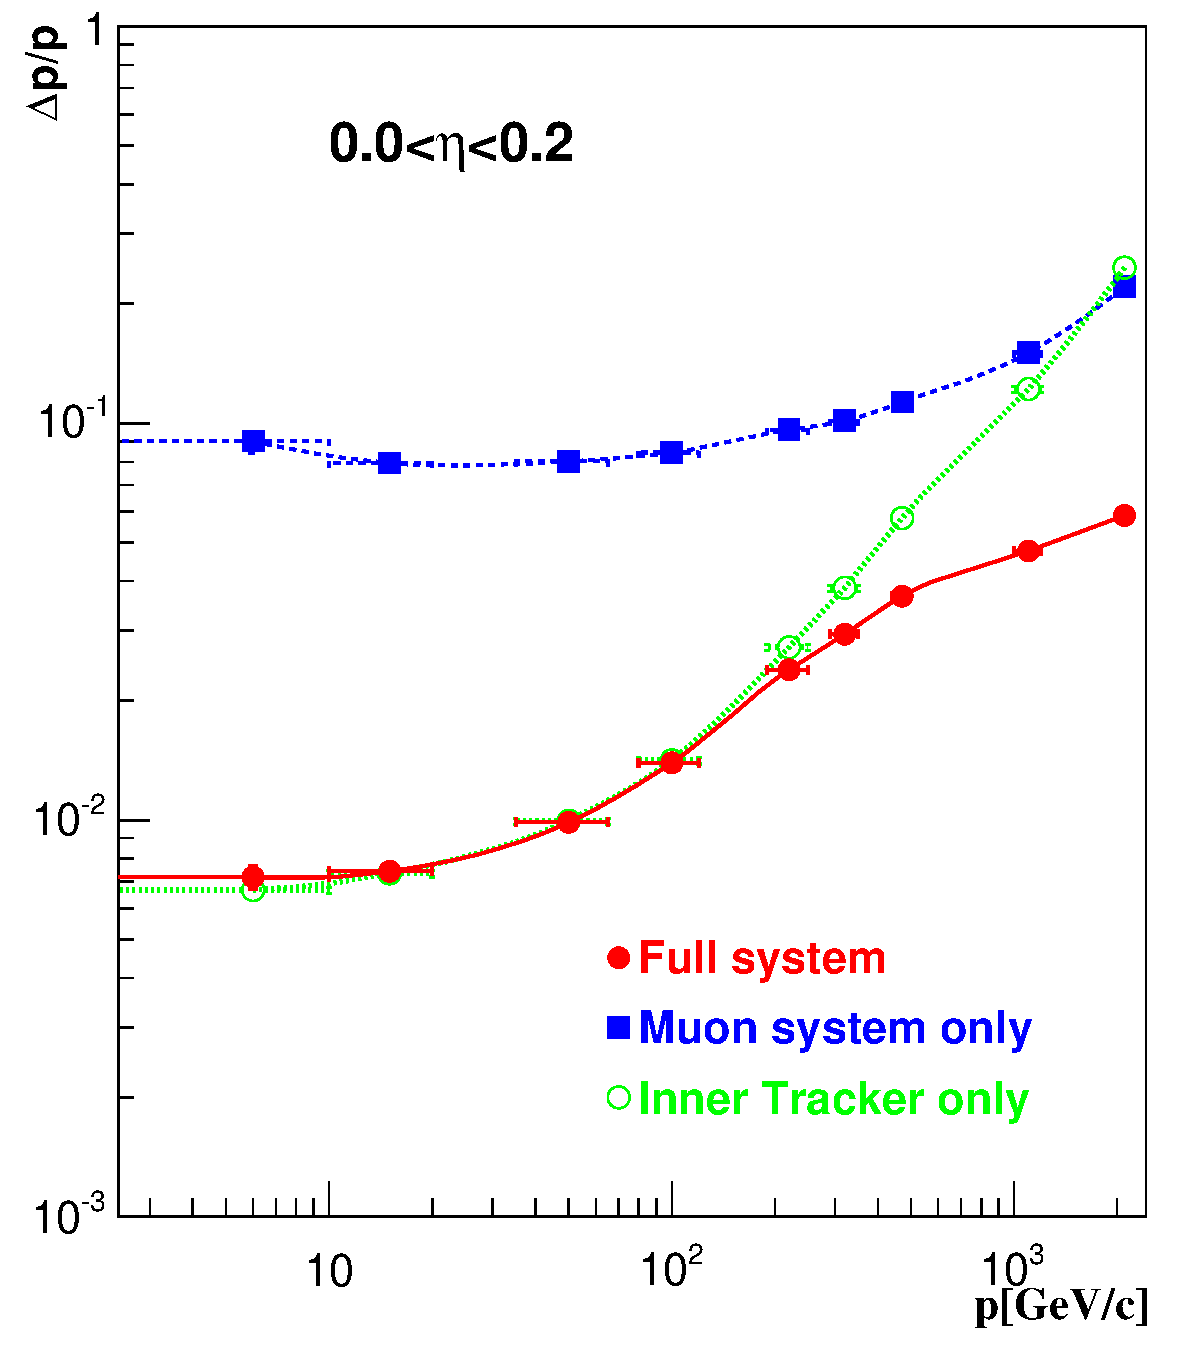
\includegraphics[width=.45\textwidth]{figures/Figure_001-005-a.pdf}
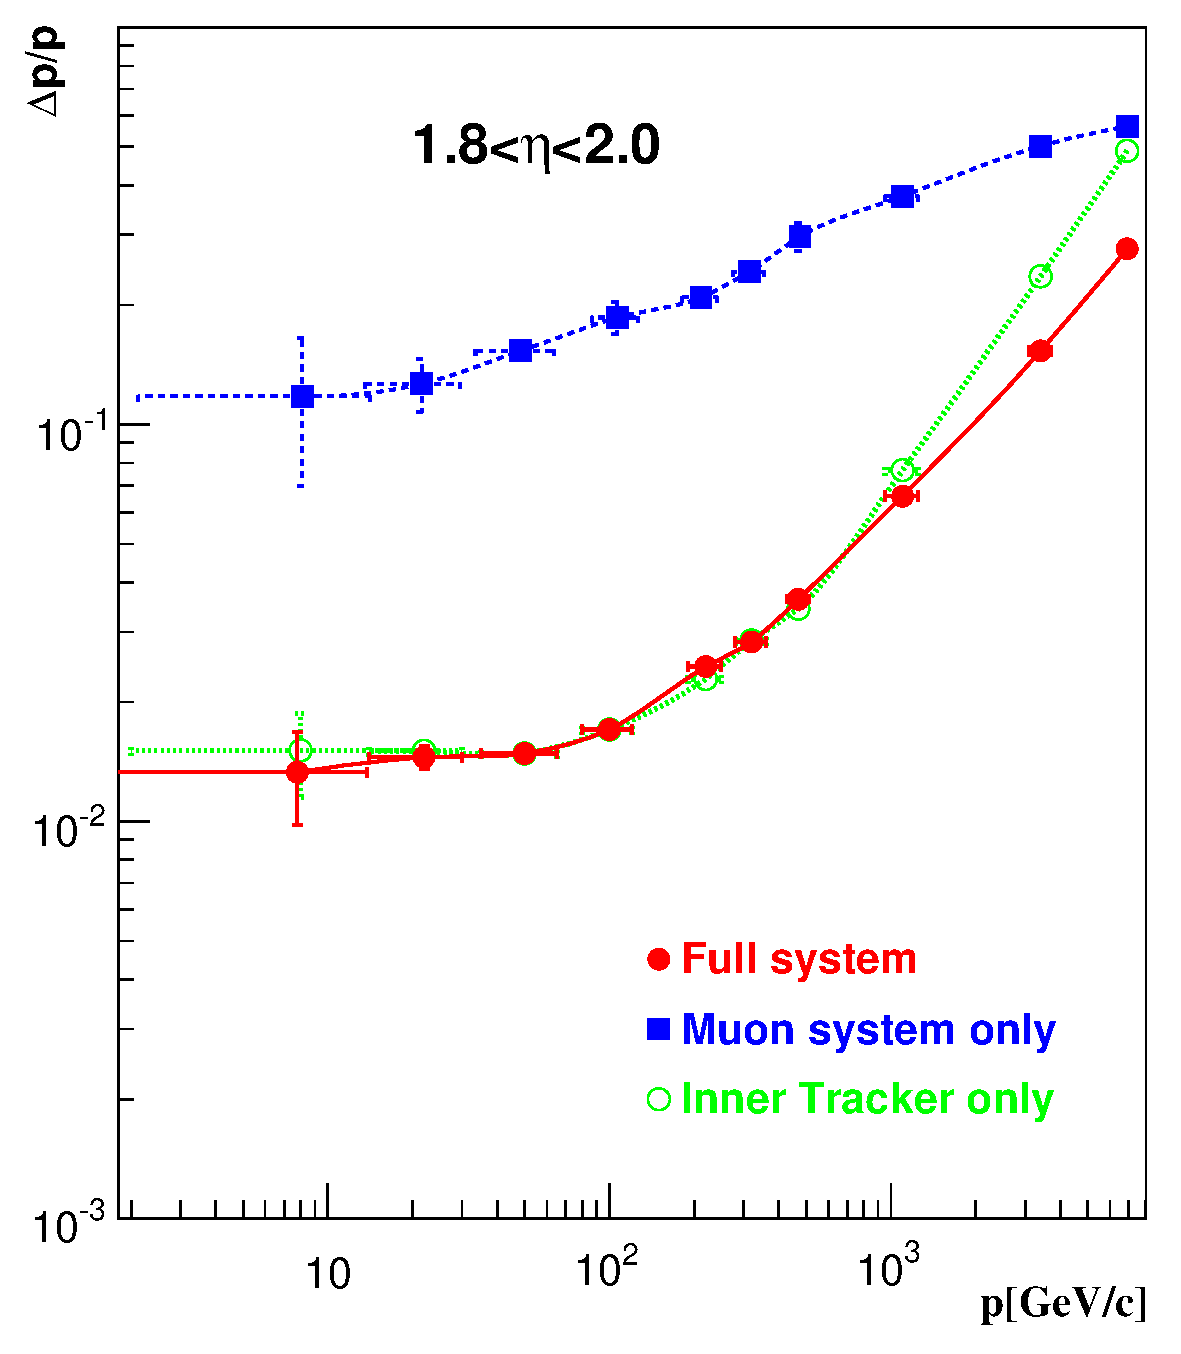
\includegraphics[width=.45\textwidth]{figures/Figure_001-005-b.pdf}
\caption{Resolution of muon momemtun in $0.0<|\eta|<0.2$ and $1.8<|\eta|<2.0$. 
Red, blue, and green are global, standalone, and tracker muons, respectively.} 
\label{fig:muon_res}
\end{figure}
Fig.~\ref{fig:muon_res} shows the momentum resolution of difference muon 
reconstruction algorithms as a function of muon \pt in the barrel(left) and endcap(right). 
The resolution of standalone muons is dominated by mutiple scattering in the material 
before the muon station at $\pt<200~\GeV$ and and by the spacial resolution 
of the muon chambers at $\pt>200~\GeV$. The tracker muons give much better 
resolution at low \pt{}, but the resolution goes up to the same level 
with the stanalone muons at very high \pt. 

The muon selection is composed of requirements on identification, isolation, and 
impact parameters.

%identification
The muon identification requirements are as follows. 
\begin{itemize}
\item The muon should be identified as PF muon 
\item $\pt>10~\GeV$ and $|\eta|<2.4$ 
\item $N_{\textrm{track layers}}>5$ 
\item $N_{\textrm{pixel hits}}$
\item $\displaystyle \frac{\delta \pt}{\pt} < 0.1$  
\item $\displaystyle \frac{\chi^2_{\textrm{kink finder}}}{\textrm{ndof}} < 20$
\item The muon should be global muon or tracker muons  
\end{itemize}
where $N_{\textrm{track layers}}$ is the number of tracker layers where the muon track has hits, 
$N_{\textrm{pixel hits}}$ is the number of pixel hits of the muon track,
$\displaystyle \frac{\delta \pt}{\pt} < 0.1$ is the relative resolution 
of the muon \pt, 
and $\displaystyle \chi^2_{\textrm{kink finder}}/\textrm{ndof}$ is the quality 
of kink finder algorithm which finds muons from decay-in-flights.  
In addtion to these requirements, the muons are required to be the global muons with 
$\chi^2/\textrm{ndof}<10$ on the global fit, 
having at least one muon hit matching the global fit 
\textcolor{red}{(what is the difference between hits and segments?)},  
and having at least two muon segments in different muon stations. 
Or, the muon can be a tracker muon satisfying that at least two muon 
segments one of which is in the outermost muon station are matched.  

%isolation 
For the isolation requirement, the MVA-based isolation variable~\cite{MuonRingIso} is used.
%to reduce contamination from non-isolated muons originating from jets. 
It uses the energy deposits of PF candidates of three categories, 
charged hadron, gamma, and neutral hadrons in the concentric isolation cones
of size $\Delta R = 0-0.1,~0.1-0.2,~0.2-0.3,~0.3-0.4,~0.4-0.5$.
Neutral components are corrected by subtracting Pileup contribution which is 
calculated by $\rho \times \textrm{A}_{\textrm{eff}}$ where $\rho$ (\texttt{kt6PFJets}) is the 
event-by-event energy density and $\textrm{A}_{\textrm{eff}}$ is the effective area.  
Effective areas are from Fall 11 simulation (\texttt{kMuEAFall11MC}) and 
values are shown in Table~\ref{tab:muAeff}.  
Exact definition of input variables to the MVA is the following. 
\begin{itemize}
\item PF charged hadron
	\begin{itemize}
    \item minimum of $\textrm{Iso}_\textrm{PF charged, 01}/\pt$ and 2.5	
    \item minimum of $\textrm{Iso}_\textrm{PF charged, 12}/\pt$ and 2.5	
    \item minimum of $\textrm{Iso}_\textrm{PF charged, 23}/\pt$ and 2.5	
    \item minimum of $\textrm{Iso}_\textrm{PF charged, 34}/\pt$ and 2.5	
    \item minimum of $\textrm{Iso}_\textrm{PF charged, 45}/\pt$ and 2.5	
	\end{itemize}
\item PF gamma : If negative, 0.0 is assigned
	\begin{itemize}
    \item minimum of $\left[\textrm{Iso}_\textrm{PF gamma, 01} - \rho \times \textrm{A}_{\textrm{eff}}\right]/\pt$ and 2.5 
    \item minimum of $\left[\textrm{Iso}_\textrm{PF gamma, 12} - \rho \times \textrm{A}_{\textrm{eff}}\right]/\pt$ and 2.5 
    \item minimum of $\left[\textrm{Iso}_\textrm{PF gamma, 23} - \rho \times \textrm{A}_{\textrm{eff}}\right]/\pt$ and 2.5 
    \item minimum of $\left[\textrm{Iso}_\textrm{PF gamma, 34} - \rho \times \textrm{A}_{\textrm{eff}}\right]/\pt$ and 2.5 
    \item minimum of $\left[\textrm{Iso}_\textrm{PF gamma, 45} - \rho \times \textrm{A}_{\textrm{eff}}\right]/\pt$ and 2.5 
	\end{itemize}
\item PF neutral hadron : If negative, 0.0 is assigned
	\begin{itemize}
    \item minimum of $\left[\textrm{Iso}_\textrm{PF neutral, 01} - \rho \times \textrm{A}_{\textrm{eff}}\right]/\pt$ and 2.5 
    \item minimum of $\left[\textrm{Iso}_\textrm{PF neutral, 12} - \rho \times \textrm{A}_{\textrm{eff}}\right]/\pt$ and 2.5 
    \item minimum of $\left[\textrm{Iso}_\textrm{PF neutral, 23} - \rho \times \textrm{A}_{\textrm{eff}}\right]/\pt$ and 2.5 
    \item minimum of $\left[\textrm{Iso}_\textrm{PF neutral, 34} - \rho \times \textrm{A}_{\textrm{eff}}\right]/\pt$ and 2.5 
    \item minimum of $\left[\textrm{Iso}_\textrm{PF neutral, 45} - \rho \times \textrm{A}_{\textrm{eff}}\right]/\pt$ and 2.5 
	\end{itemize}
\end{itemize}
where we defined 
\begin{eqnarray} 
\textrm{Iso}_\textrm{PF,XY} 
= 
\sum_{
\begin{subarray}{l}
\textrm{PF candidates in the cone of} \\
\textrm{0.X}   < \Delta R^{\mu-\textrm{PF candidate}} < \textrm{0.Y} 
    \end{subarray} }
\pt
%\textrm{the scalar sum of \pt\ of PF candidates in the cone of 0.X} 
%< \Delta R^{\mu-\textrm{PF candidate}} < \textrm{0.Y}.
\end{eqnarray} 
We require that the MVA output be greater than 0.82 (0.86) in $10<\pt~<20~\GeV$ 
and 0.86 (0.82) in $\pt~>20~\GeV$. The cut values correspond to the ones in barrel (endcap).

\begin{table}[htp]
	\centering
		\begin{tabular}{c|c|c|c|c|c|c}
			\hline 
				\multicolumn{7}{c}{PF gamma} \\
	  	    \hline
			 	$|\eta|$     & $0.0 - 1.0$ & $1.0 - 1.479$ & $1.479 - 2.0$ & $2.0 - 2.2$ & $2.2 - 2.3$ & $2.3-$ \\       		
	  	    \hline \hline
				$0.0<dR<0.1$ & 0.004& 0.002& 0.003& 0.009& 0.003& 0.011 \\
				$0.1<dR<0.2$ & 0.012& 0.008& 0.006& 0.012& 0.019& 0.024 \\
				$0.2<dR<0.3$ & 0.026& 0.020& 0.012& 0.022& 0.027& 0.034 \\
				$0.3<dR<0.4$ & 0.042& 0.033& 0.022& 0.036& 0.059& 0.068 \\
				$0.4<dR<0.5$ & 0.060& 0.043& 0.036& 0.055& 0.092& 0.115 \\
	  	    \hline \hline 
				\multicolumn{7}{c}{PF neutral hadron} \\
	  	    \hline 
			 	$|\eta|$     & $0.0 - 1.0$ & $1.0 - 1.479$ & $1.479 - 2.0$ & $2.0 - 2.2$ & $2.2 - 2.3$ & $2.3-$ \\       		
	  	    \hline \hline
				$0.0<dR<0.1$ & 0.002& 0.004& 0.004& 0.004& 0.010& 0.014 \\
			    $0.1<dR<0.2$ & 0.005& 0.007& 0.009& 0.009& 0.015& 0.017 \\
			    $0.2<dR<0.3$ & 0.009& 0.015& 0.016& 0.018& 0.022& 0.026 \\ 
				$0.3<dR<0.4$ & 0.013& 0.021& 0.026& 0.032& 0.037& 0.042 \\ 
				$0.4<dR<0.5$ & 0.017& 0.026& 0.035& 0.046& 0.063& 0.135 \\ 
			\hline
		\end{tabular}
		\caption{ Effective areas used for muon isolation. They were calculated with Fall11 MC sample.}
	\label{tab:muAeff}
\end{table}

%impact parameter 
In addtion, we apply require transverse/longditudinal impact parameters 
to be associated with the event primary vertex. 
The transverse impact parameter is required 
to be less than 0.01 cm for $\pt<20~\GeV$ and 0.02 cm for $\pt>20~\GeV$. 
The longitudinal impact parameter is required to be less than 0.01 cm. 

The efficiency of the full muon selection measured in MC is \textcolor{red}{XX} \% 
for electrons from HWW 125 and \textcolor{red}{YY} \% for electrons from W+jets.  


%%%%%%%%%%%%%%%%%%%%%%%%%%%%%%%%%%%%%%%%%%%%%%%%%%%%%%%%%%%%%%%%%%
\section{ Jet }
\label{sec:jetselection}
\begin{itemize}
\item \textcolor{red}{Jet reconstruction : anti-kT (dR = 0.5) }
\item \textcolor{red}{Jet energy correction : L1Fastjet/L2/L3 (+ Residual correction in data) }
\item \textcolor{red}{lepton veto ($dR>0.3$) }
\item \textcolor{red}{MVA jet ID(list of input variables, training samples, cut values)}
\item \textcolor{red}{two definitions : (1) jet bin counting($\pt>30~\GeV$) (2) top veto($10<\pt<30~\GeV$) }
% have a plot like this for MVA Jet ID? not sure how I drew this though
% maybe a script is somewhere on uaf
%http://uaf-2.t2.ucsd.edu/~jaehyeok/HWW/PhilJetIDMVA/dev/PhilJetIDMVAefssssssss.pdf
\end{itemize}

The existence of gluons and quarks in the event is manifested as a hadronic shower, 
``jets", which leaves an energy deposit primarily in the HCAL. 
Thanks to the fine granuality of CMS detector system, individual hadrons can 
be reconstructed by PF algorithm. 
The, jets are reconstructed with PF candidates using anti-$\textrm{k}_\textrm{T}$ algorithm \cite{}
with a cone size $\Delta R$ = 0.5. Due to the non-linear calorimeter response of CMS detector, 
the measured jet energy can not be translated into the energy of the true parton which 
initiated the jet. CMS employs jet energy correction(JEC) method \cite{} factorized into 
several levels, L1, L2, L3 and residual corrections for data. 
The L1 correction is the PileUp/noise correction, \textit{i.e.} to remove offset energy 
from PileUp and noise. The correction is composed of two sub-correction, 
one from the real jet energy loss due to detector thresholds and 
the other from PileUp. The offset energy in a jet area is measured as a function 
of \Eta{} in the zero-bias and min-bias samples.    
The L2 correction is to make the jet energy response flat in \Eta.  
At a given \Eta{} response is corrected so that the it becomes at the same level 
of the central region, $|\Eta|<1.3$. So, the correction is relative. 
The correction factors are derived from either MC or using data-driven method
(di-jet balance \cite{}).
The L3 correction is to make the jet energy response flat in \pt.  
The central region, $|\Eta|<1.3$, is used as a referece for the correction. 
Apart from the L2 correction, L3 correction is an absolute correction 
such that the corrected jet \pt{} is same as the \pt{} of the parton that 
initiated the jet. The correction factors are derived from either MC 
or using data-driven method($Z/\gamma^*$+jet balance \cite{}). 
For L2 and L3 corrections, the corrections based on MC truth is done for MC 
and residual corrections are applied to data to account for the small differences 
between data and MC. 

Jets fot this analysis are selected first by rejecting overlaps with selected electrons 
and muons. If the $\Delta R$ between a lepton and the jet is less than 0.3, the jet 
is very likely to be a lepton, thus it is rejected. In high PileUp environment, 
clustering random PF particle from PileUp interactions can lead to a high \pt{} jet. 
To suppress this noise, we apply MVA-based PileUp jets suppression techique. 
Jets from pileup are soft, so they need to be overlaid to pass the jet $\pt$ threshold. 
Therefore, energy deposit of pileup jets are more spread than the one from hard interactions.
We select jets of which MVA outputs are greater than the values 
which correspond to the loose working point in Table~\ref{tab:jetidcut}.
\begin{table}[htp]
	\centering
		\begin{tabular}{c|c|c|c|c}
			\hline
									&  $0<|\eta|<2.5$ 	& $2.5<|\eta|<2.75$		& $2.75<|\eta|<3.0$ 	& $3.0<|\eta|<4.7$ 		\\ 
			\hline \hline
				$\pt<10$ \GeV		& 0.0 				& 0.0					& 0.0	 				& 0.2					\\ 
				$10<\pt<20$	\GeV 	& -0.4 				& -0.4					& -0.4	 				& 0.4					\\
				$20<\pt<30$	\GeV	& 0.0 				& 0.0					& 0.2	 				& 0.6					\\ 
				$\pt>30$ \GeV 		& 0.0 				& 0.0					& 0.6	 				& 0.2					\\
			\hline 
		\end{tabular}
		\caption{Cut values on jet identification MVA outputs. MVA output is required to be greater than 
				these values to be counted as a jet.}
	\label{tab:jetidcut}
\end{table}
Of the selected jets, the high \pt{} jets ($\pt>30~\GeV]$ and $|\Eta|<4.7$) are used for counting 
the number of jets, and the low \pt{} jet ($10<\pt<30~\GeV]$ and $|\Eta|<4.7$) are used 
for rejecting top events. 
\textcolor{red}{Any plots to show? MVA values for real jet and PU jets? or JEC factorization? 
look at the slides I made for jet MVA id, there's veto efficiency as a function of Nvtx.} 
\begin{figure}[!hbtp]
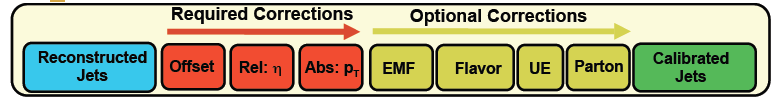
\includegraphics[width=.99\textwidth]{figures/jecfactoriztiontmp.png}
\end{figure}


%%%%%%%%%%%%%%%%%%%%%%%%%%%%%%%%%%%%%%%%%%%%%%%%%%%%%%%%%%%%%%%%%%
\section{ Missing Transverse Energy }
\begin{itemize}
\item \textcolor{red}{How MET(pfMET and trackMET) is calculated } 
\item \textcolor{red}{mention MET $\phi$ modulation correction }
\item \textcolor{red}{define projected MET (compare signal and bkgd, (ex) \ztt)}
\item \textcolor{red}{cut values ($\textrm{minMET} > 20~\GeV$) }
\end{itemize}
There are some particles that do not interact with materials. One of them is neutrino.
When neutrinos are produced at the collider, they do not leave any signature 
in the detector, so they can not be reconstructed. However, we can infer 
the existence of neutrino, or any weakly-interacting particles, by computing 
the imbalance in the vector sum of transverse momenta of the reconstructed particles.
The transverse momentum of the initial particles is zero 
\footnote{It is not perfectly zero because partons have transverse movements 
inside the proton. But, the energy of their motion is at most a few hundred \MeV{}
which is much less than the resolution of measurements.}.
By momentum convervation, the total momentum of the particles produced 
after collision should be 0 as well. 
So, if the transverse momenta of all particles in the final state are summed up, 
the negative value of the vector sum should correspond to the transverse momentum 
sum of neutrinos. Thus, we define ``Missing Transverse Energy(\met)", 
\begin{eqnarray} 
\overrightarrow{\met} = - \sum^{\textrm{All PF candidates}}_i \overrightarrow{\pt}(i).
\end{eqnarray} 
In this analysis, \met{} is calculated with particles reconstructed using PF algorithm.

The $\phi$ distribution of true \met{} should be flat because of the rotational 
symmetry of collisions with respect to the beam axis. However, possibly due to 
anisotropic detector response, inactive calorimeter response, detector misalignments, 
and displacement of the beam spot, the $\phi$ distributions of \met{} in both 
MC and data are not flat, but a sinusoidal shape with a period $2\pi$. 
Thus, we correct this by shifting the origin of the coordinates 
in the transverse momentum plane for x and y components individually. 
Since the size of the shift increases 
linearly as a function of number of reconstructed primary vertices, 
the form of correction is given by 
\begin{eqnarray} 
\alpha + \beta N_{\textrm{vertex}}
\end{eqnarray} 
where $\alpha$ and $\beta$ shown in Table~\ref{tab:metxycorrection} are constants 
and $N_{\textrm{vertex}}$ is the number of primary vertices. 
\begin{table}[htp] 
\begin{center} 
\begin{tabular}{c||c|c|c} 
\hline 
                       &                  & $\alpha$ &  $\beta$  \\
\hline \hline 
\multirow{2}{*}{MC}    & correction for X & $-3.00 \times 10^{-2}$ & $-6.62\times 10^{-2}$  \\
                       & correction for Y & $3.71\times 10^{-1}$   & $-1.49\times 10^{-1}$  \\
\hline 
\multirow{2}{*}{Data}  & correction for X & $3.54\times 10^{-1}$   & $2.65\times 10^{-1}$   \\
                       & correction for Y & $1.89\times 10^{-1}$   & $1.66\times 10^{-1}$   \\
\hline 
%    metx -= (+3.54233e-01 + 2.65299e-01*nvtx_);
%    mety -= (+1.88923e-01 - 1.66425e-01*nvtx_);
%    metx -= (-2.99576e-02 - 6.61932e-02*nvtx_);
%    mety -= (+3.70819e-01 - 1.48617e-01*nvtx_);
\end{tabular} 
\caption{Parameters used for XY shift correction for \met.} 
\label{tab:metxycorrection} 
\end{center} 
\end{table} 
\textcolor{red}{optional : show the met distribution before/after the correction}


The \met{} is used to reject processes which do not have true source of missing energy. 
Target processes are QCD and \dyll{} where \met{} comes from primarily due to 
mis-measurement of jet momentum. However, in case of \dytt{}, the \Tau{} can 
decay into lepton and neutrinos, giving true missing momentum. Because of large 
mass difference between Z and \Tau{}, \Tau{} is generally boosted significantly 
with its decay products flying in the same direction of the \Tau momentum. 
Therefore, the missing energy component perpendicular to the lepton momentum 
is a better measure for true \met{} which is originated from \Tau{} decays. 
To realize this we define ``projected \met " (\pmet) as 
\begin{equation}
\pmet 
= 
\begin{cases} \met & \text{if $\Delta\phi_{min}>\frac{\pi}{2}$,}
\\
\met\sin(\Delta\phi_{min}) & \text{if $\Delta\phi_{min}<\frac{\pi}{2}$}
\end{cases}
\end{equation}
where  
\begin{equation}
\Delta\phi_{min} =  min(\Delta\phi(\ell_1,\met),\Delta\phi(\ell_2,\met)).
\end{equation}
The $\Delta\phi(\ell_i,\met)$ is the angle between \met{} and the lepton $i$ 
on the transverse plane. Figure~\ref{fig:projmetscheme} shows the schematic 
of \pmet. 
\begin{figure}[htp] 
\centering 
\begin{tabular}{c} 
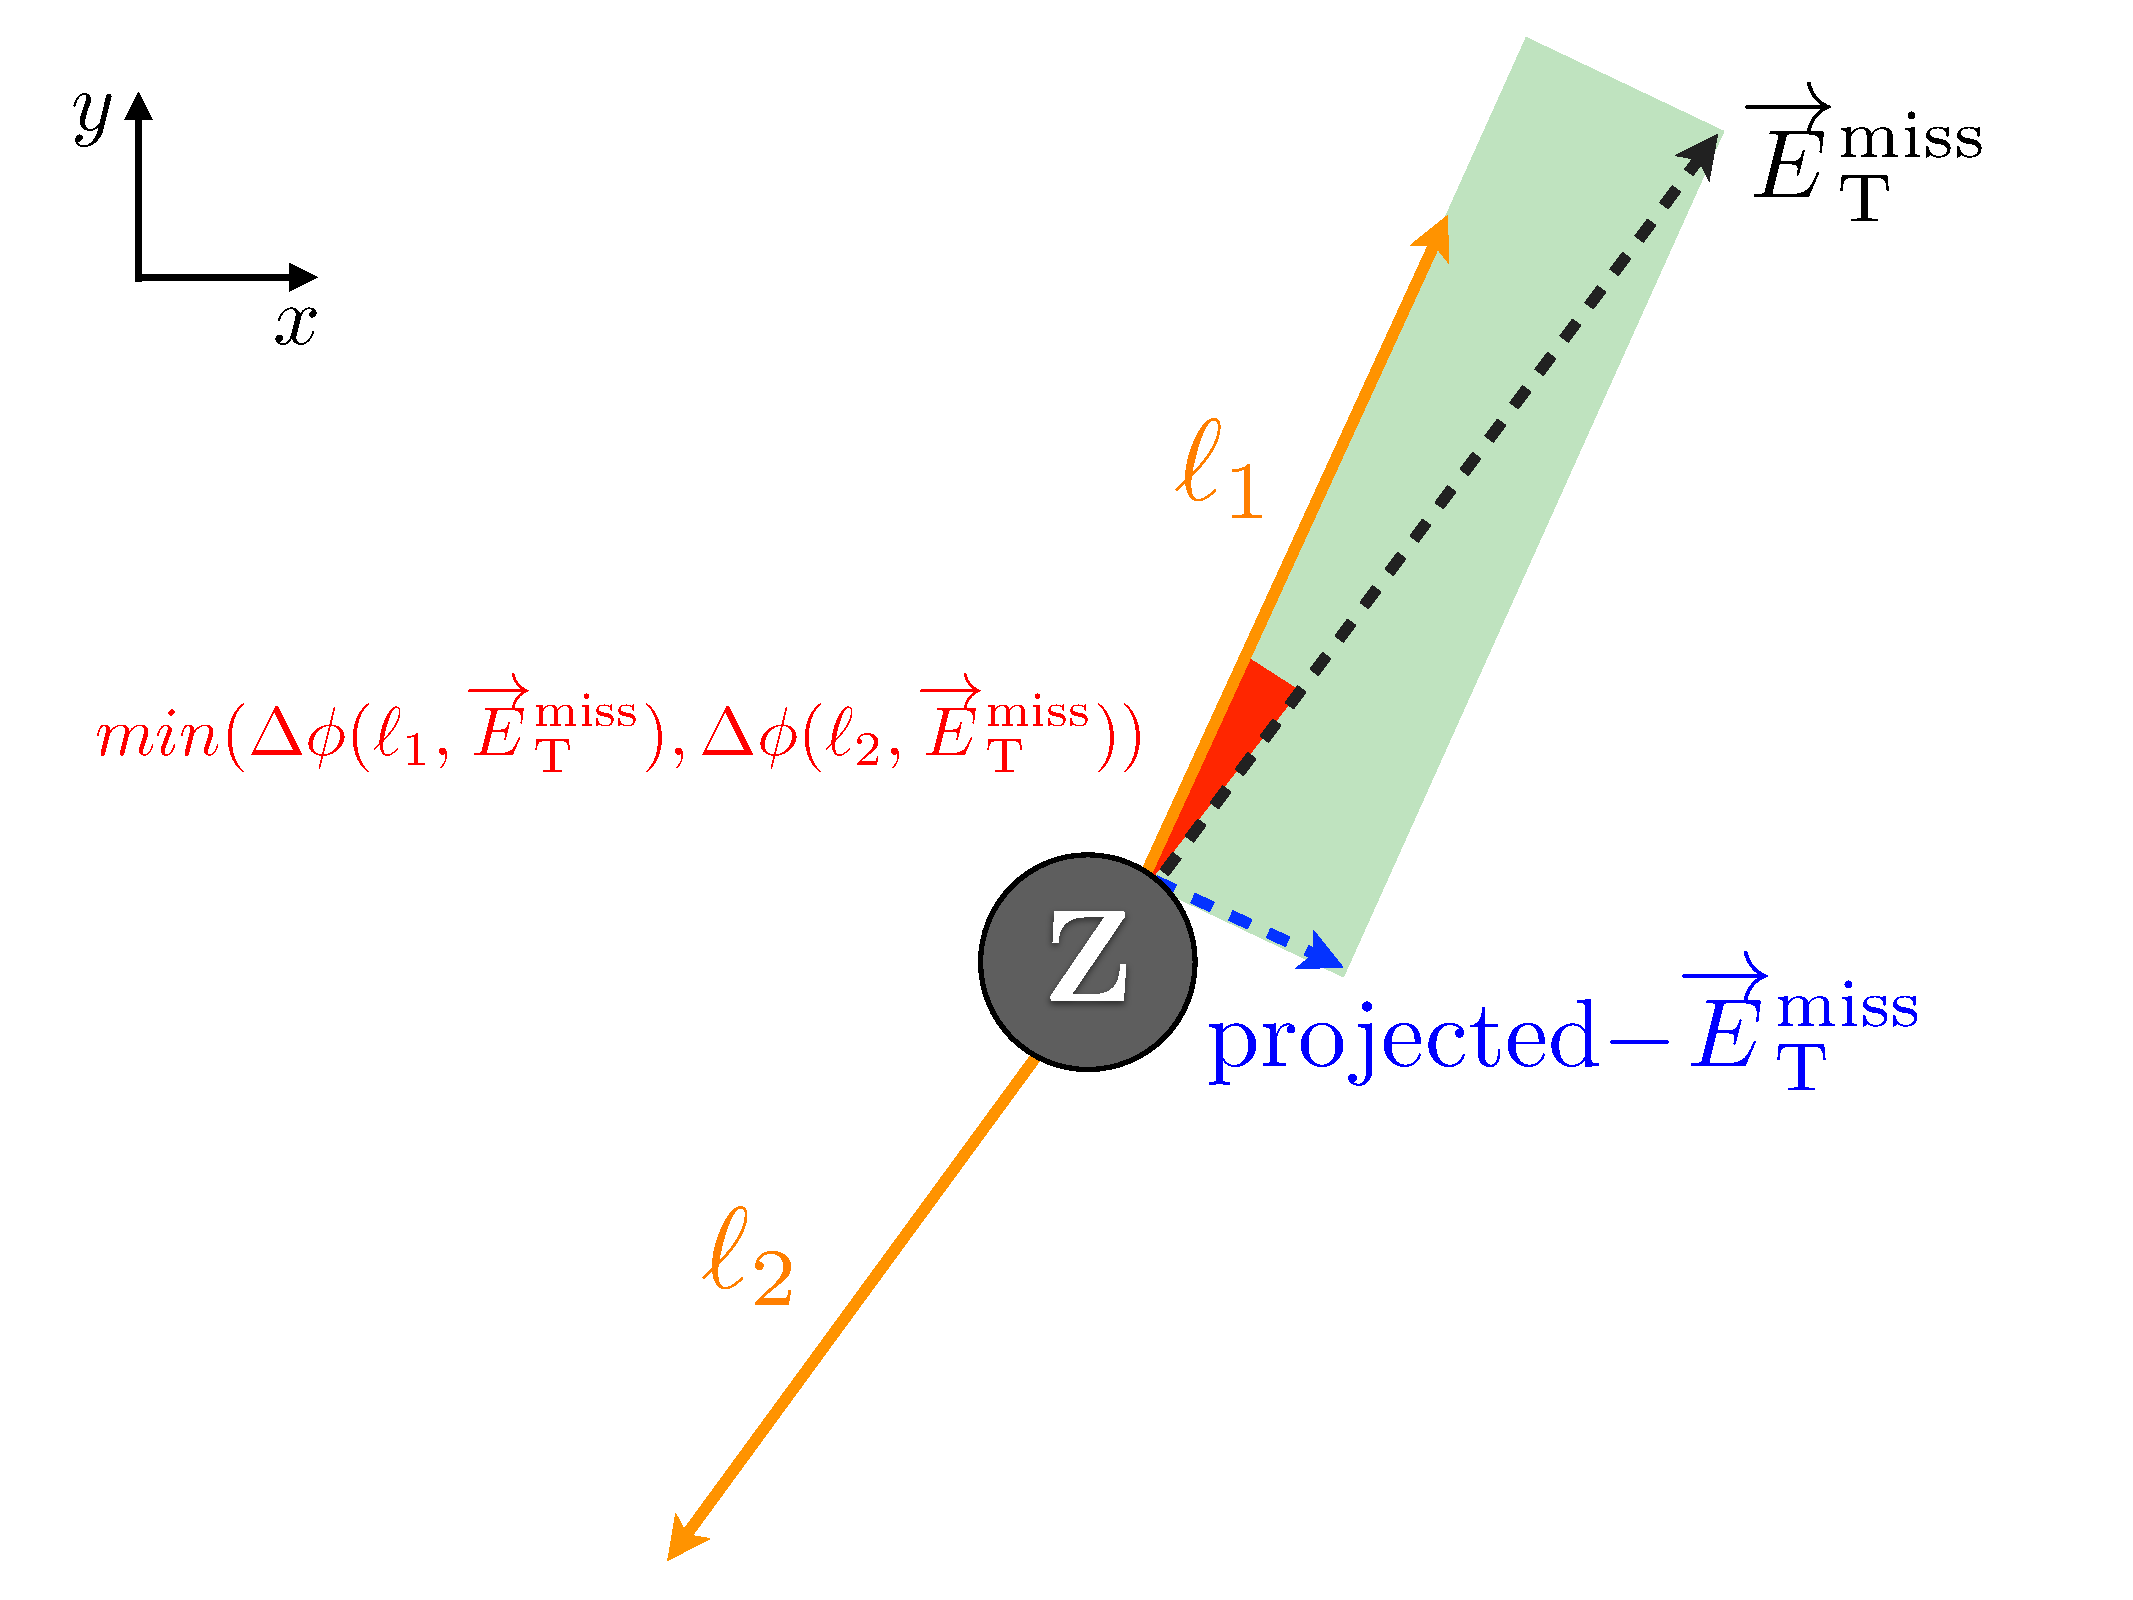
\includegraphics[width=0.7\textwidth]{figures/projmet.pdf} 
\end{tabular} 
\caption{Schematic of \pmet.}
\label{fig:projmetscheme} 
\end{figure}  
%
\begin{figure}[htp] 
\centering 
\begin{tabular}{c} 
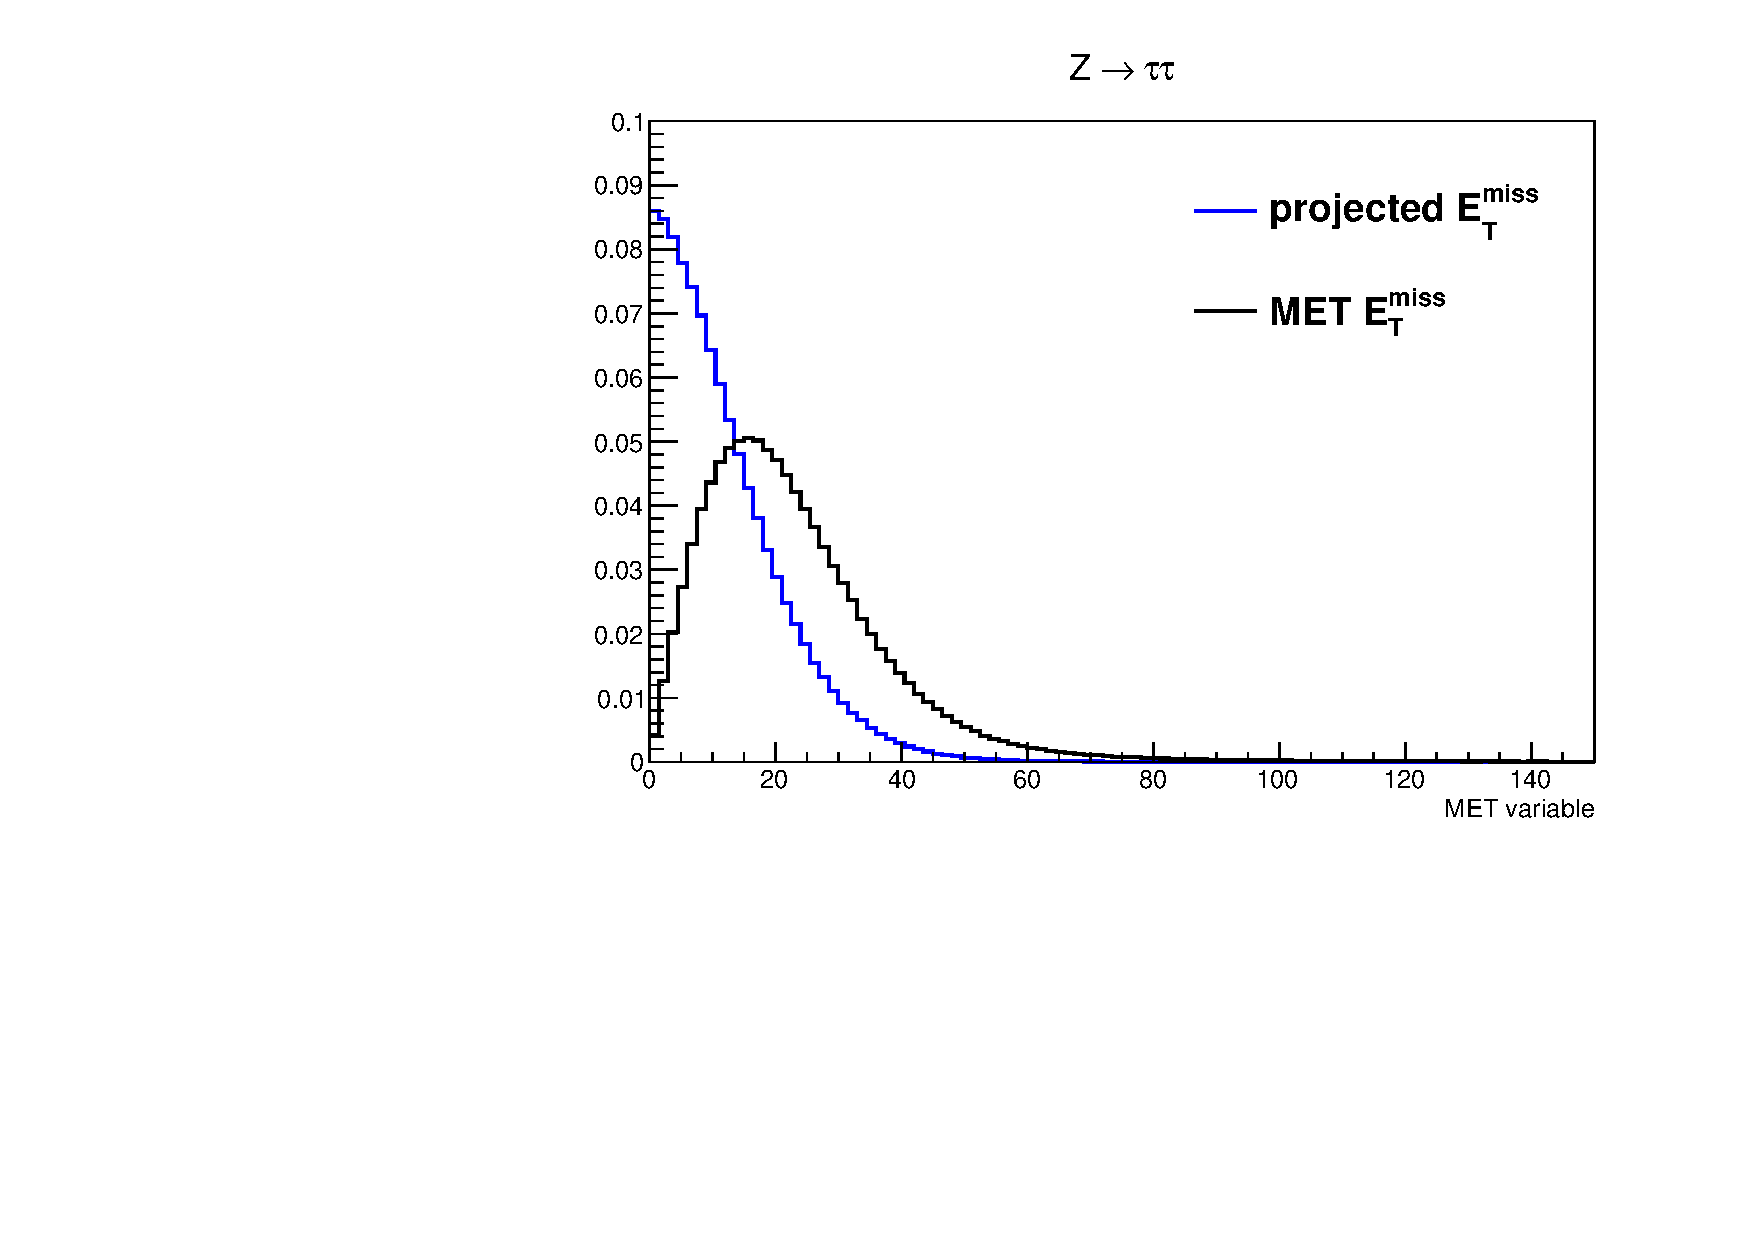
\includegraphics[width=0.45\textwidth]{figures/pmet_met_ztt.pdf} 
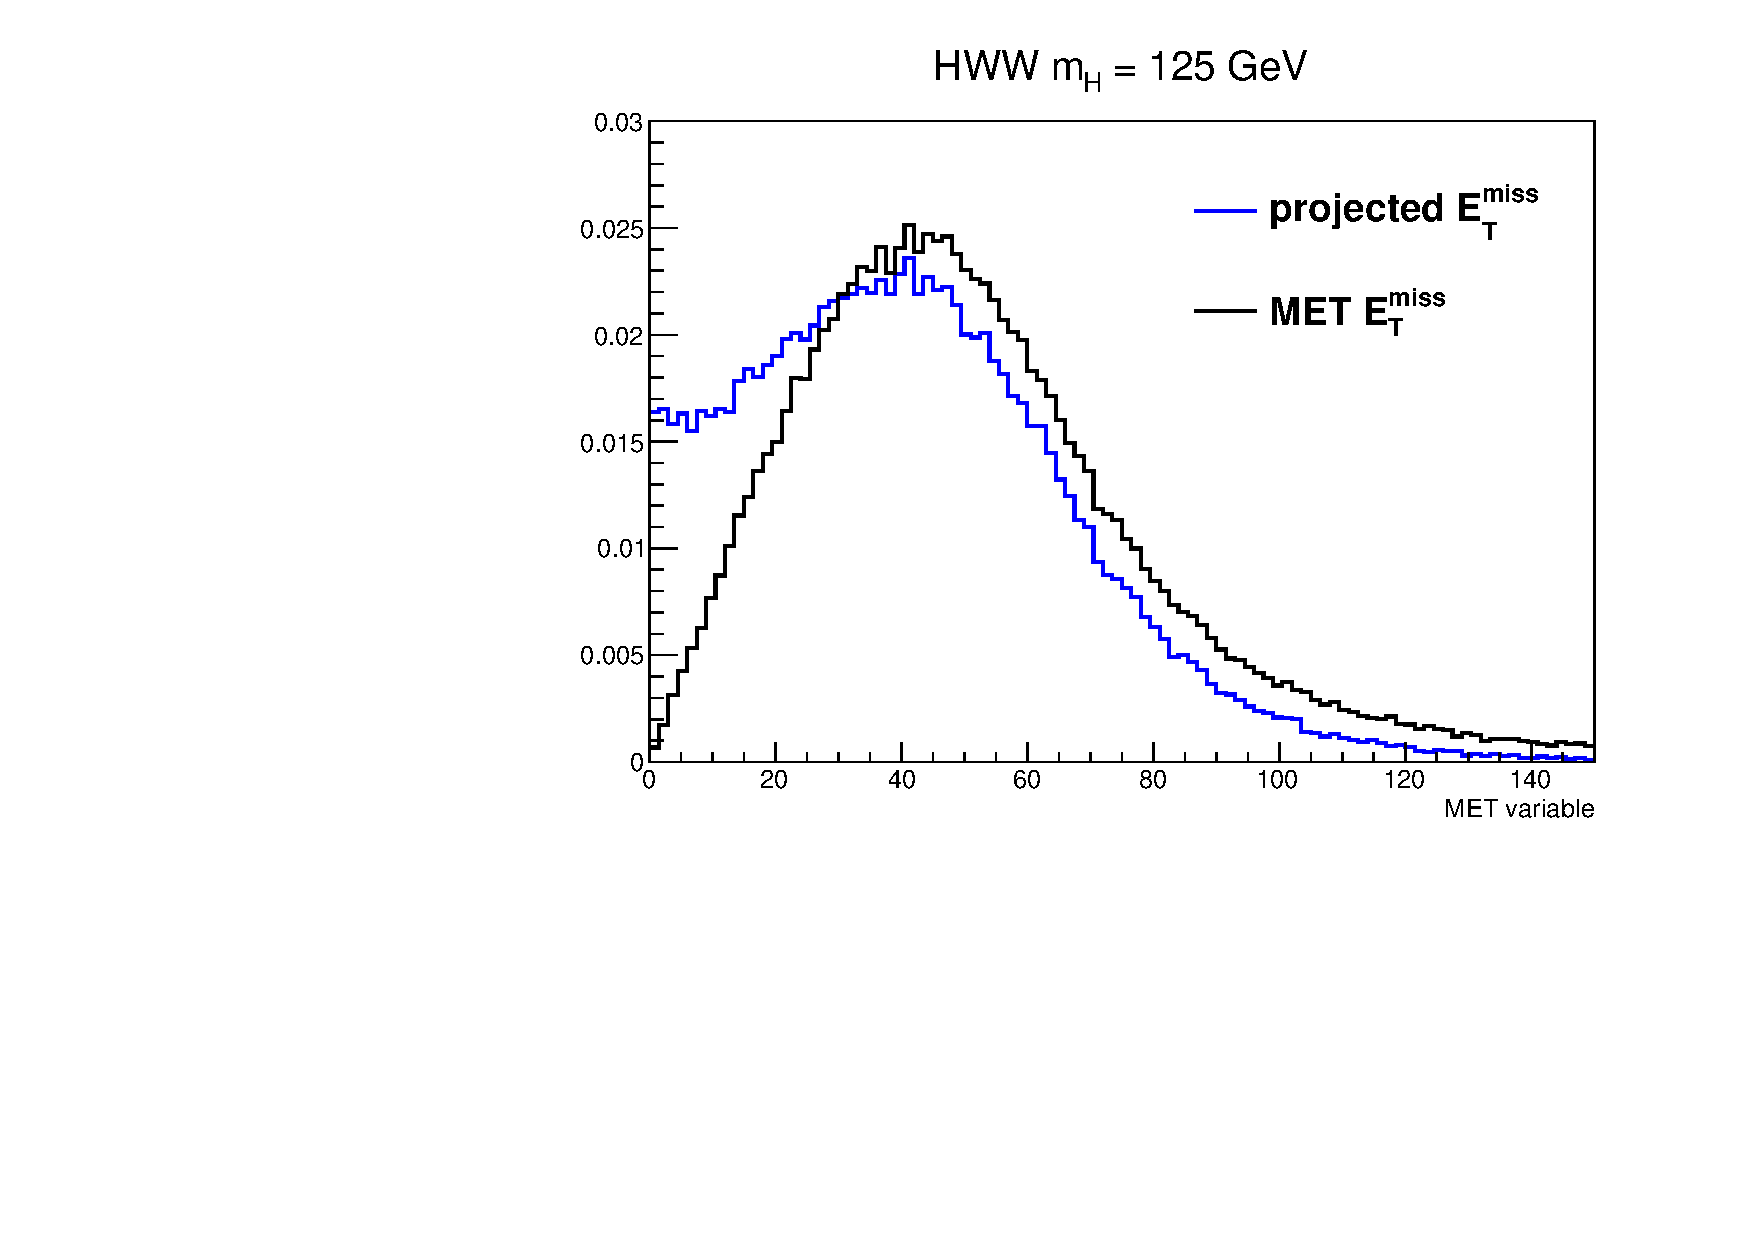
\includegraphics[width=0.45\textwidth]{figures/pmet_met_hww125.pdf} 
\end{tabular} 
\caption{\met(black) and \pmet(blue) in \dytt{}(left) and SM Higgs at \mHi=125~\GeV(right).}
\label{fig:projmet} 
\end{figure}  
Figure~\ref{fig:projmet} shows the \met{} and the \pmet{} distributions 
in black and red, repectively, in \dytt{} and SM Higgs at \mHi=125~\GeV 
on left and right, repectively. We can see that \pmet is more squeezed to 
the lower values in case of \dytt, giving better rejection power.  

The performance of met reconstruction is degraded in high luminosity environment 
because of random contribution from paricles from PileUp to the \met{} calculation. 
So, we use another definition of \met{} which is calculated with only charged 
PF candidates associated with the event primary vertex. Since particles from 
other vertices that the event primary vertex are excluded in the \met{} calculation,
the \met{} calculated using this method is independent of number of PileUps.  
This \met{} definition is called ``\trkmet" and exact definition is
\begin{eqnarray} 
\overrightarrow{\trkmet} 
= 
- \overrightarrow{\pt} (\ell_1)  
- \overrightarrow{\pt} (\ell_2)  
- \sum^{\textrm{All charged PF candidates}}_i \overrightarrow{\pt}(i)
\end{eqnarray} 
where $\overrightarrow{\pt} (\ell_1)$ and $\overrightarrow{\pt} (\ell_2)$
are the transverse momemta of the leptons. The charged PF candidates must 
meet the following requirements.
\begin{itemize}
\item The longitudinal impact parameter of the track matched to the PF candidate 
      with respect to the event primary vertex should be less than 0.1~cm. 
\item $\Delta R$ between the track matched to the PF candidate and the leptons 
      should be larger than 0.1 in order to avoid counting leptons twice. 
\end{itemize}
There is an issue of \trkmet{} which is that its tail is longer than \pfmet 
in \dyll{} events. This is due to the imbalance of neutral and charged hardrons 
in the jets. By isospin symmetry the average number of neutral particles($\pi^0$) should 
be a half of charged particles($\pi^\pm$). If \textcolor{red}{..... finish the reasoning.....}  
The the correlation between the two definitions is strong in the events with 
true \met, and weak in the events with fake \met{} as shown in Fig.~\ref{fig:2dmet}. 
To protect from neutral - charged imbalance and to enhance the signal vs. background 
separation power, we used minimum of the the two projected \met{} definitions, 
\minpmet, which is defined as 
\begin{eqnarray} 
\minpmet = min \left( \pmet, \ptrkmet \right). 
\end{eqnarray} 

We require \minpmet{} to be greater than 20~\GeV in all categories as a baseline selecion. 
For further rejection of \dyll{} background, we apply MVA-based technique which will be 
discussed in detail in section~\ref{sec:dybkg}. 

%
\begin{figure}[htp] 
\centering 
\begin{tabular}{c} 
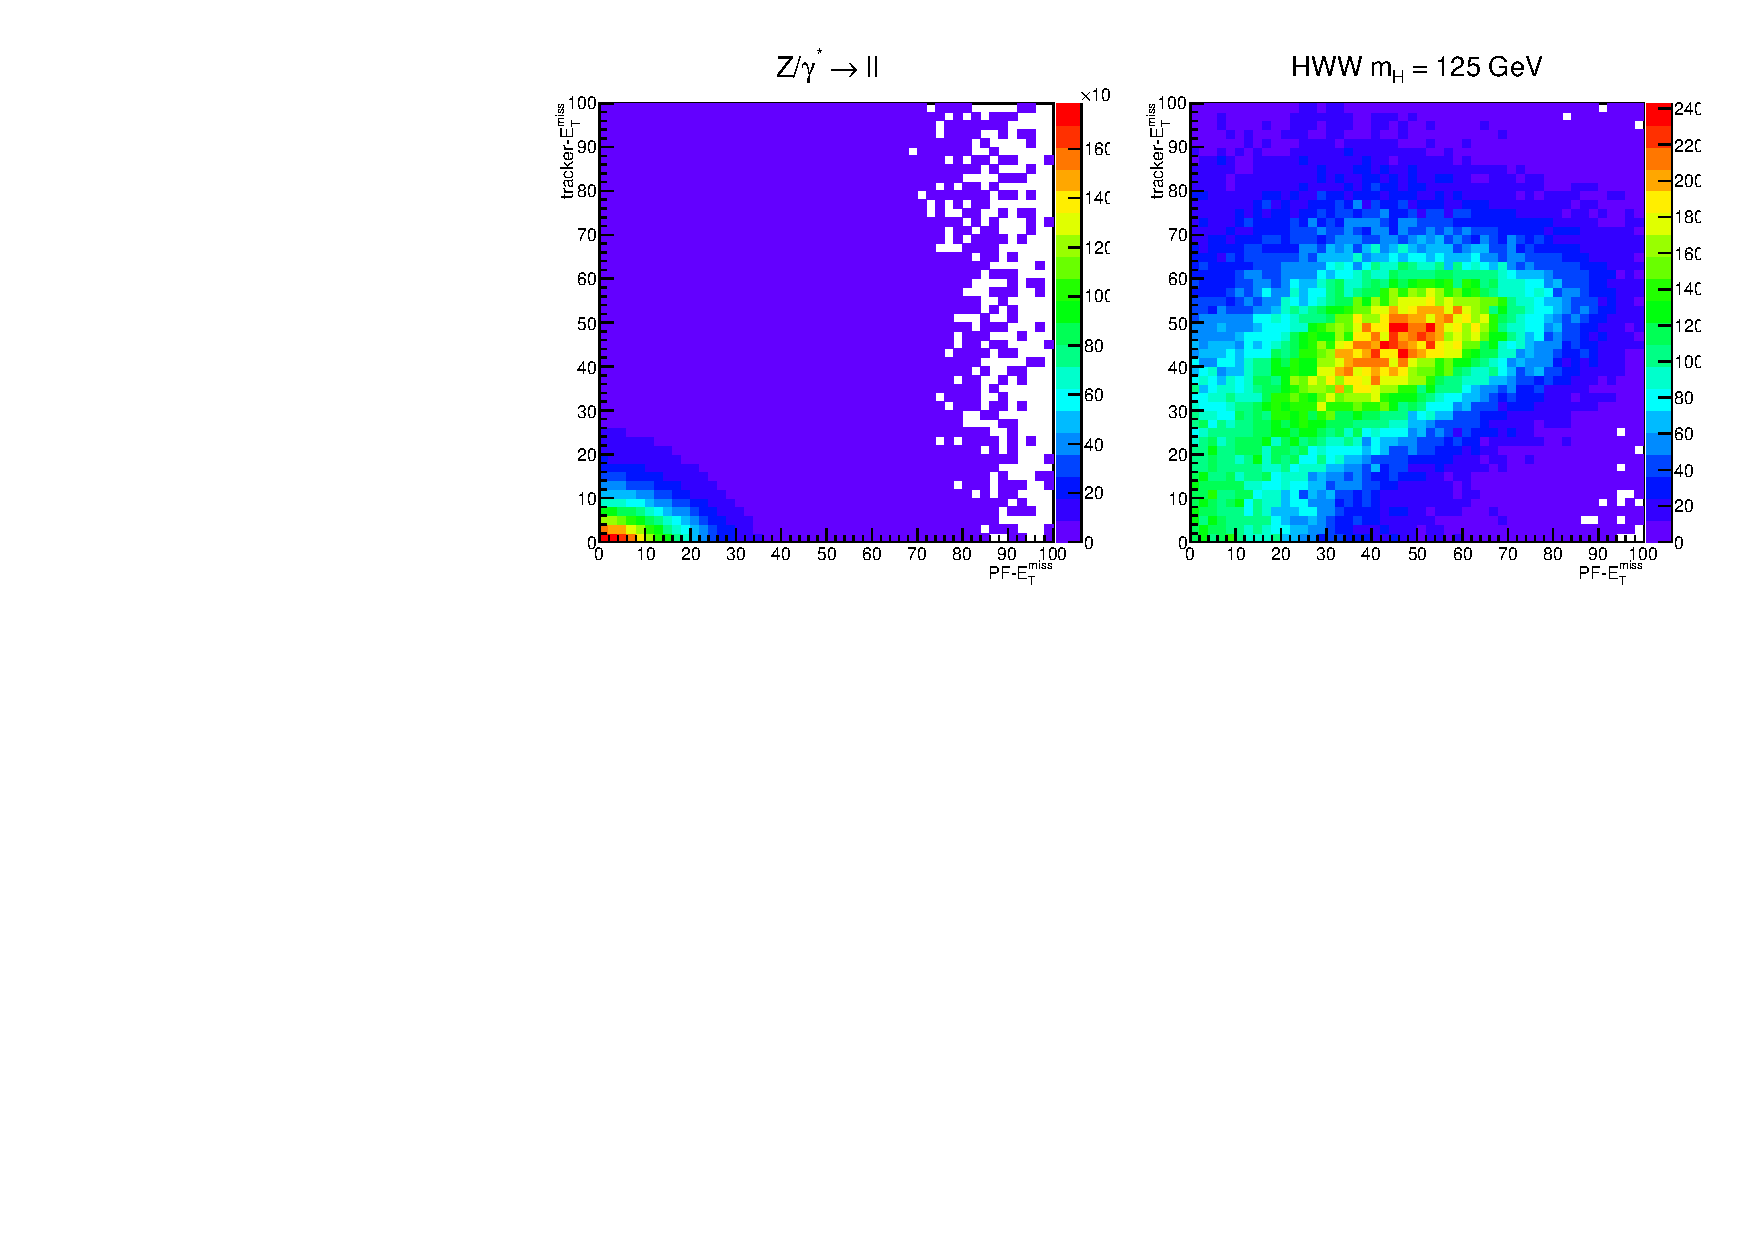
\includegraphics[width=0.99\textwidth]{figures/2dmet.pdf} 
\end{tabular} 
\caption{\pmet{} vs. \ptrkmet{} in \dyll{} and SM Higgs \mHi = 125~\GeV.}
\label{fig:2dmet} 
\end{figure}  

%%%%%%%%%%%%%%%%%%%%%%%%%%%%%%%%%%%%%%%%%%%%%%%%%%%%%%%%%%%%%%%%%%
\section{ Top-tagging }
\begin{itemize}
\item \textcolor{red}{How B-tagging algorithm works and working point
      (TCHEM : Track Counting High Efficiency Medium)}
\item \textcolor{red}{how the discriminating variable is calculated }
\item \textcolor{red}{quote some performance plots }
\item \textcolor{red}{soft-muon tagging requirement }
\end{itemize}

The presence of a bottom quark in the event is manifested by the presence a secondary vertex. 
The bottom quark is hadronized to a B meson($\textrm{B}^0, \textrm{B}^\pm, ...$) and it 
traverses for a measurable distance before decaying into other particles.
Typically, the b-tagging algorithms use information of the impact parameter(IP) of 
charged particles decayed from the B meson or the distance between the primary vertex 
and the secondary vertex. 
\begin{figure}[htp] 
\centering 
\begin{tabular}{c} 
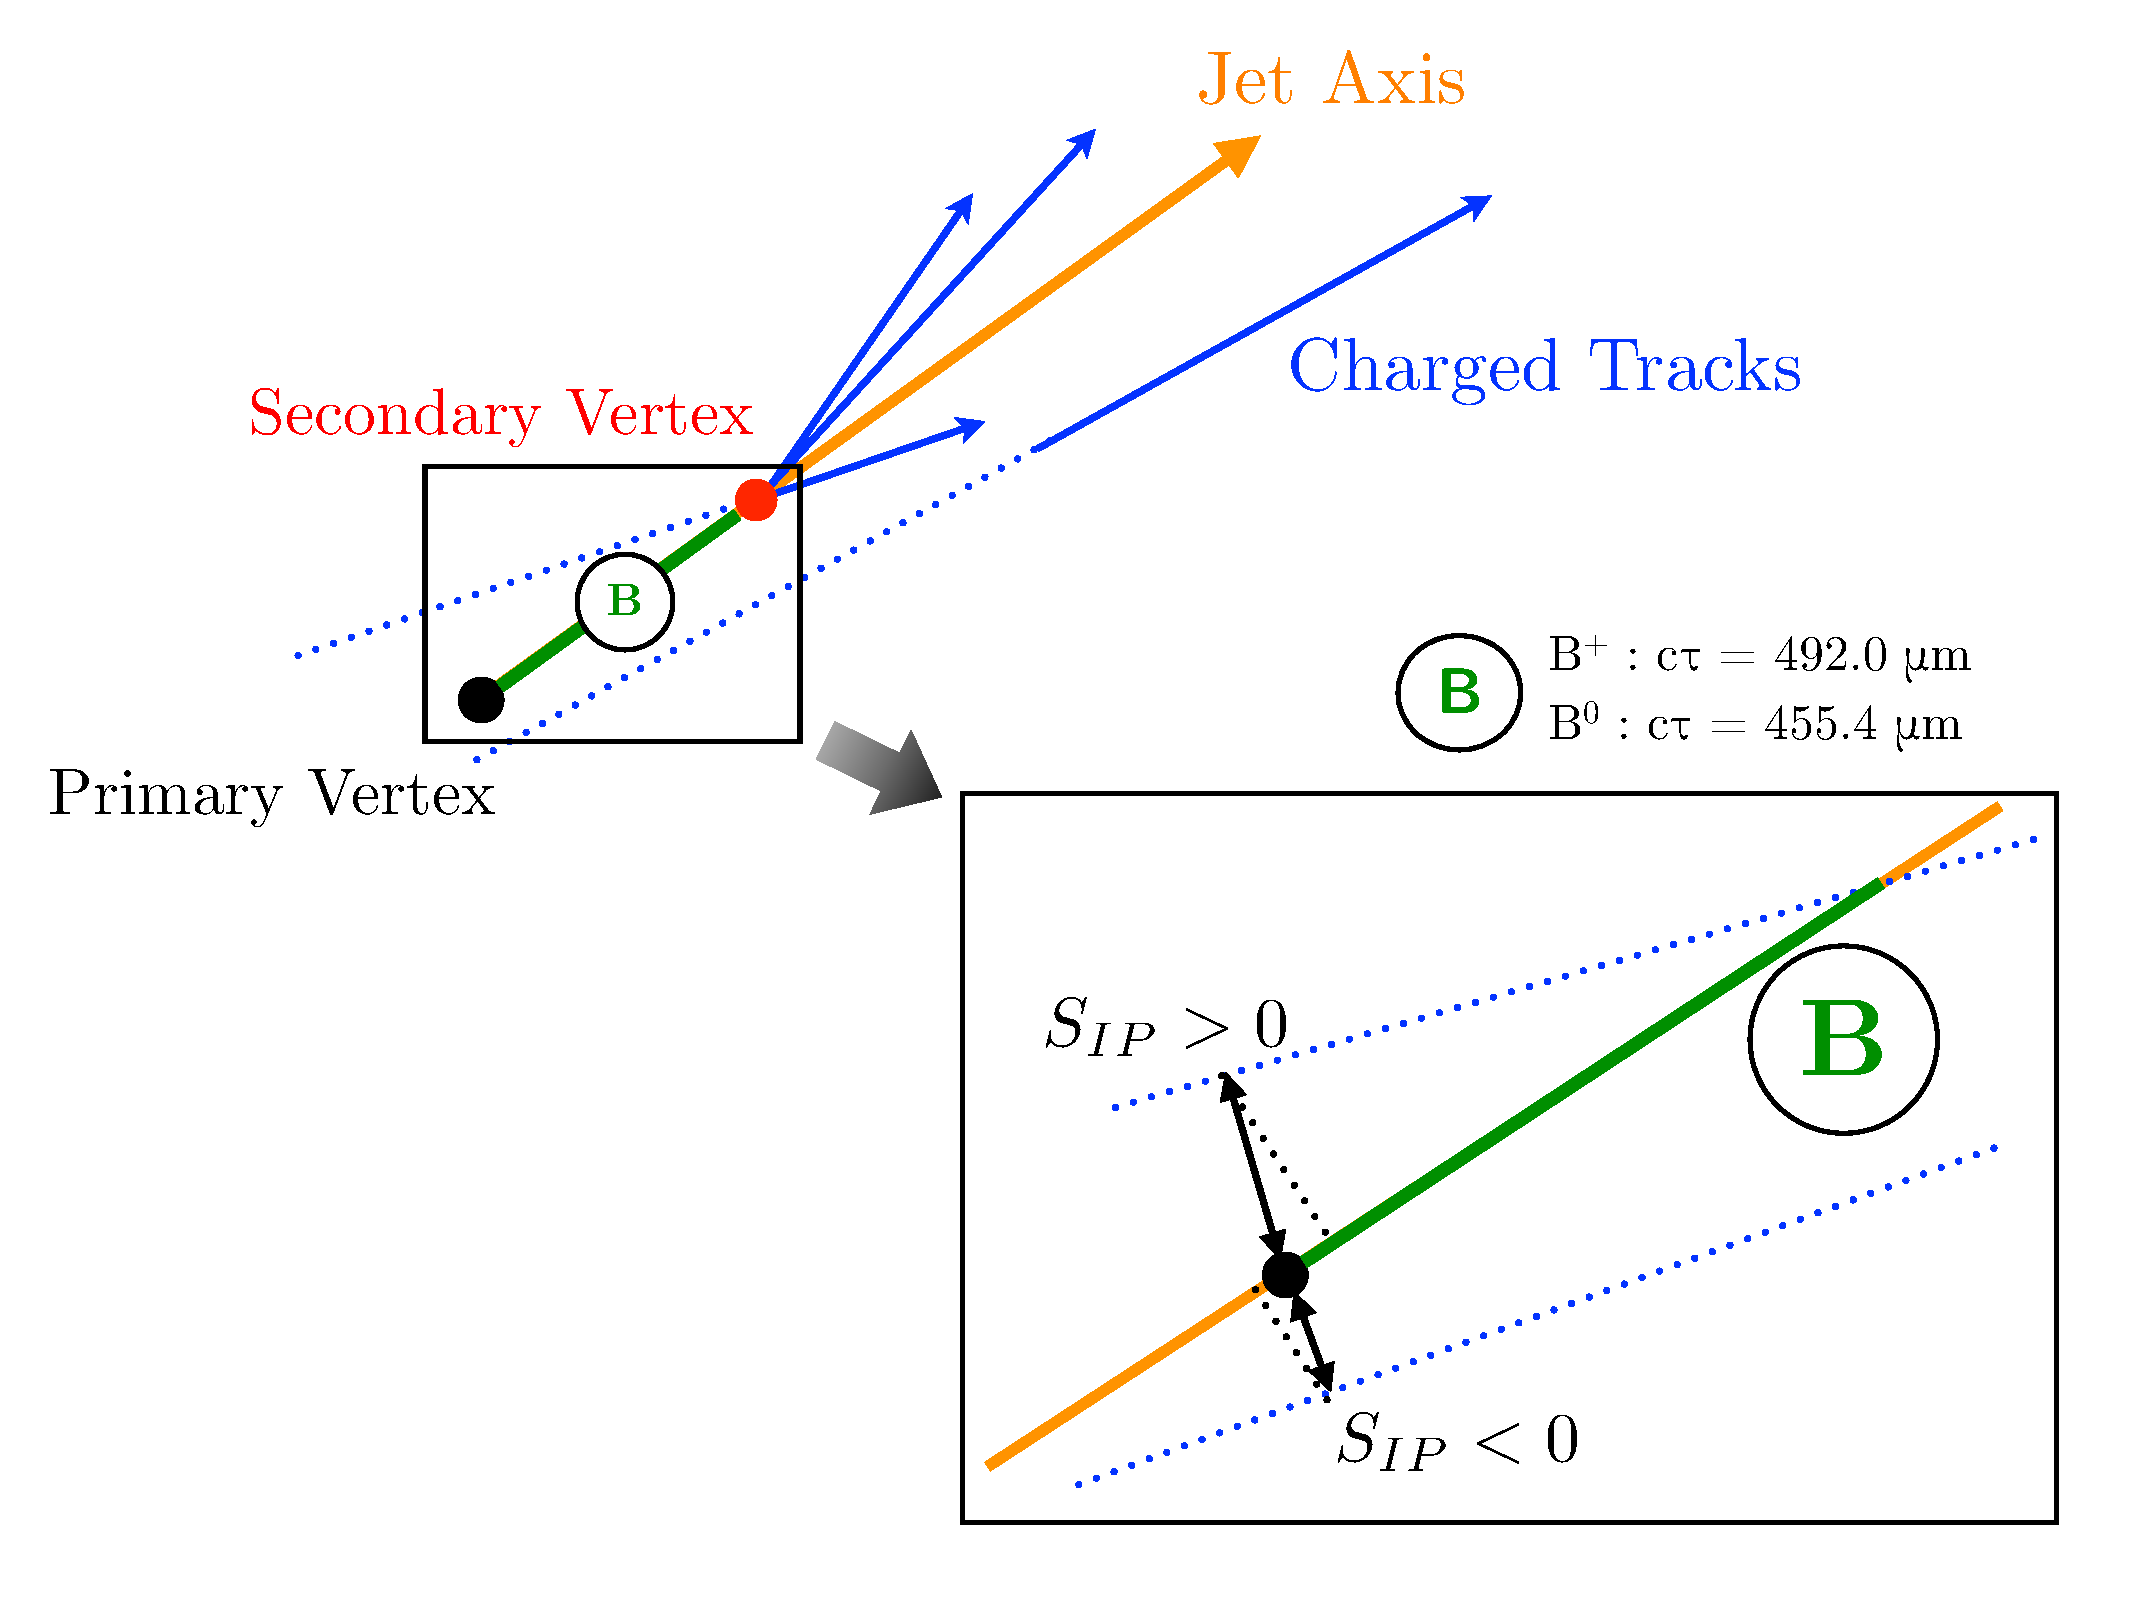
\includegraphics[width=0.99\textwidth]{figures/Btag.pdf} 
\end{tabular} 
\caption{A schematic of b-taging algorithm.}
\label{fig:btag} 
\end{figure} 
The IP is calculated in 3D thanks to the good z resolution of the 
pixel detector. The IP can be signed depending on the position of 
the associated track. The sign is obtained from the sign of the scalar product of 
IP vector from the primary vertex and the direction of the jet the track belongs to
as shown in Fig.~\ref{fig:btag}.
For the decays with sizable lifetime, the IP should be positive in theory, 
but it is not always positive in case the real direction of the B meson 
is different from the direction of the jet. But, they still tend to be positive. 
For the decays with very short lifetiem or random tracks that happen to be 
considered for btagging algorithm, the IP is symmetric around 0.   

In b-tagging algorithm used in this analysis is so called ``TrkCountingHighEff(TCHE)" \cite{}.
This algorithm uses the impact parameter significance, $S_{IP} = IP / \sigma_{IP}$ 
where $\sigma_{IP}$ is the uncertainty of the IP measurement, 
as a discribinating variable. The algorithm requires at least 2 tracks to have $S_{IP}$ 
above a given threshold. Thus, the discriminator is the $S_{IP}$ of the second highest 
significance. 
If the b-tagging descriminator of a jet with $\pt>10~\GeV$ that passes the criteria described in
section~\ref{sec:jetselection} is greater than 2.1, this jet is selected as a b-tagged jet. 
Finally, to suppress \topbkg{} backgrounds, events with at least one b-tagged jets are rejected. 
\textcolor{red}{show MC vs Data of the discriminating variable in the top control region?}

We enhance the rejection of \topbkg{} backgrounds by rejecting events that contain 
non-isolated soft muons from heavy flavor decays. The following requirements are imposed to 
select soft muons. 
\begin{itemize} 
    \item $\pt > 3~\GeV$ 
    \item The muon should be a tracker muon
    \item The muon should have at least two muon segments one of which is 
          in the outermost muon station are matched.
    \item $N_{\textrm{track layers}}>5$ 
    \item $|d_{0}| < 0.2$~cm;
    \item $|d_{z}| <0.2$~cm;
    \item ${\rm{Iso}_{\textrm{Total}}}/{\pt}>0.1$ if $\pt>20~\GeV$.
\end{itemize} 
where $N_{\textrm{track layers}}$ is the number of tracker layers where the muon track has hits, 
$d_{0}$($d_{z}$) are the transverse(longitudinal) impact parameter with respect to 
the event primary vertex, and $\rm{Iso}_{\textrm{Total}}$ is the sum of \Et{} inside of the cone 
with $dR < 0.3$ in ECAL and HCAL, and \pt{} of tracker. Adding soft muon requirement 
especially helps in the 0-jet category where the top rejection efficiency increases 
about 50 \% compared to using b-tagging only.

The total top rejection efficiency using both methods when applied to \topbkg{} MC 
is about 50 \% in the 0-jet category and 80 \% in the 1-jet category. 



